%% The first command in your LaTeX source must be the \documentclass command.
%%
%% Options:
%% twocolumn : Two column layout.
%% hf: enable header and footer.
\documentclass[letterpaper,11pt]{article}
\usepackage{amsmath, amsthm, amssymb}
\usepackage{bridges}
\usepackage{graphicx}

\usepackage[colorlinks=true, urlcolor=blue, citecolor=black, linkcolor=black]{hyperref}
\usepackage{subcaption}



\usepackage{algorithm}
\usepackage{algpseudocode}
\usepackage{hyperref}

%\usepackage{svg}
\usepackage{multirow}
\usepackage{caption}
\usepackage{tikz}

\usepackage[bottom]{footmisc}

\urlstyle{rm}


%%
%% One can fix some overfulls
\sloppy

%%
%% Minted listings support 
%% Need pygment <http://pygments.org/> <http://pypi.python.org/pypi/Pygments>
\usepackage{listings}

%% auto break lines
\lstset{breaklines=true}

\title{ A Generalized 2D and 3D Hilbert Curve }
\author{ Jakub \v{C}erven\'{y} and Zzyv Zzyzek }
%\author[]{Jakub \v{C}erven\'{y}}[%
url=https://github.com/jakubcerveny,
]
\author[]{Zzyv Zzyzek}[%
%url=https://zzyzek.github.io,
orcid=0009-0005-2175-1166,
]


\date{}

%%
%% Rights management information.
%% CC-BY is default license.
%\copyrightyear{2026}
%\copyrightclause{Copyright for this paper by its authors.
%  Use permitted under Creative Commons License Attribution 4.0
%  International (CC BY 4.0).}


%%
%% end of the preamble, start of the body of the document source.
\begin{document}

\maketitle

%%
%% This command is for the conference information
%\conference{EXAG 2024: AIIDE Workshop on Experimental AI in Games, November 18--22, 2024, Lexington, KY, USA}
%\input{CONFERENCE.tex}


\begin{abstract}
  The two and three dimensional Hilbert curves are fractal space filling curves that
  map the unit interval to the unit square or unit cube while preserving a notion
  of closeness, or locality, after the map.
  We present the Gilbert curve,
  a conceptually straight forward generalization of the Hilbert curve,
  that works on arbitrary rectangular regions, overcoming the limitation of the Hilbert
  curve that requires side lengths be exact powers of two.
  Our construction of the Gilbert curve provides a notion of \textit{harmony}
  that provide alternate subdivision schemes when a side length is much larger than the rest,
  creating more visual pleasing curves as a result.


%The construction provides reasonable worst case run-time guarantees for random
%access lookups for both two and three dimensions.
%We provide experiments showing comparable quality in locality of the Gilbert curve
%to the Hilbert curve for a range of cuboid regions and discuss some limitations of
%  the construction algorithm.
\end{abstract}


%\newcommand{\specialcell}[2][c]{\begin{tabular}[#1]{@{}l@{}}#2\end{tabular}}
%\newcommand{\specialcellCenter}[2][c]{\begin{tabular}[#1]{@{}c@{}}#2\end{tabular}}

%  \section*{Generalized Hilbert Curves}

In a website application and scanned note \cite{lutanho2003}, Tautenhahn provided the basis for a generalized 2D
space filling curve.
Tautenhahn also included policies for when to subdivide regions preferentially in only one dimension
that help to create more \textit{harmonious} curve realizations.
Tautenhahn's exploration details the parity arguments necessary for when a subdivision scheme can be employed
without creating diagonal moves (\textit{notches}).

In this paper, we extend Tautenhahn's ideas to create a 2D and 3D generalized Hilbert curve.
We further extend Tautenhahn's core ideas on when to use alternate subdivision schemes when one length is much
larger than the rest, what we call \textit{eccentric cases}, and extend them to 3D.
Tautenhahn's unpublished reasoning behind the constants used in the 2d eccentric split case are briefly discussed
later in this paper \footnote{ Through personal communication with the authors, Tautenhahn
kindly provided the reasoning for the constants used in the eccentric split }.

\begin{figure}[!htb]

  \begin{minipage}{0.48\textwidth}

    \centering
    \includegraphics[width=\linewidth]{gilbert2d_examples.pdf}
    \caption{ 2D Gilbert curves for i) $8 \times 8$, ii) $18 \times 6$, iv) $13 \times 8$ (with notch), iv) $14 \times 14$ }
    \label{fig:gilbert2d_examples}
  \end{minipage}\hfill
  \begin{minipage}{0.48\textwidth}
    \centering
    \includegraphics[width=\linewidth]{gilbert3d_orig_examples.pdf}
    \caption{ 3D Gilbert curves for i) $4 \times 4 \times 4$, ii) $6 \times 6 \times 6$, iii) $8 \times 4 \times 4$, iv) $5 \times 4 \times 4$ (with notch) }
    \label{fig:examples3d}

  \end{minipage}

\end{figure}


\section*{Valid Paths from Grid Parity}

\begin{figure}[!htb]

  \begin{minipage}{0.48\textwidth}

    \centering
    %\begin{table}[h]
    %  \centering
      \begin{tabular}[t]{cr|cc}
        \multicolumn{2}{c}{ \multirow{2}{*}{Path Possible} } & \multicolumn{2}{c}{Volume} \\
        & & \textit{even} & \textit{odd} \\
        \hline
          %\multirow{2}{*}{$|\alpha| \bmod 2$} & \textit{even} & Yes & Yes \\
          \multirow{2}{*}{ $|\alpha|$ } & \textit{even} & Yes & Yes \\
           & \textit{odd} & \textbf{No} & Yes \\
         \hline
      \end{tabular}
      \caption{ $|\alpha|$ is the distance of endpoints.
                A Hamiltonian path is possible only when $|\alpha|$ is even or both
                $|\alpha|$ and the volume are odd. }
      \label{table:pathTable}
    %\end{table}

  \end{minipage}\hfill
  \begin{minipage}{0.48\textwidth}

    \centering
    \includegraphics[width=\linewidth]{simple_hampath.pdf}
    \caption{ Examples of Hamiltonian paths for small grid sizes. A red `x' corresponds to no possible path for the chosen endpoints. }
    \label{fig:exampleHampath}

  \end{minipage}


\end{figure}

The feasibility of determining whether there exists a Hamiltonian path connecting endpoints on the
corners in a rectangular cuboid
grid region can be accomplished through parity arguments.
Label grid cell points in a volume as 0 or 1,
alternating between labels with every axis-aligned single step move.
Any Hamiltonian path that ends at one of the three remaining corners has to have the same parity as the starting point if the
volume is odd, or different parity if the volume is even.


For a path starting at $(0,0,0)$ and ending $|\alpha|$ steps in one of the axis-aligned dimensions,
then Table \ref{table:pathTable} enumerates this condition under which a valid path is possible.
Figure \ref{fig:exampleHampath} illustrates this for starting position $(0,0)$ with areas $(2 \times 2)$, $(3 \times 2)$ and $(3 \times 3)$,
where a red cross indicating a precluded endpoint.

Without loss of generality, we will assume a curve starts from position $p_s=(0,0,0)$ and has proposed
endpoint at $p_e=((w-1),0,0)$, with a cuboid region as $\alpha = (w,0,0), \beta = (0,h,0), \gamma = (0,0,d)$.
We state, without proof, that
a Hamiltonian path is always possible from $p_s$ to $p_e$ when $|\alpha|$ is even or when all of $|\alpha|$, $|\beta|$ and $|\gamma|$
are odd  $(|\alpha| \cdot (1 - |\beta| \cdot |\gamma|) \equiv 0 \bmod 2)$.

When the condition $(|\alpha| \cdot (1 - |\beta| \cdot |\gamma|) \equiv 0 \bmod 2)$ is met ($|\alpha|$ even or all of $|\alpha|, |\beta|, |\gamma|$ odd)
any cuboid subdivision will always have a Hamiltonian path feasible within it.
We can recreate a Hamiltonian path in the larger cuboid region by connecting neighboring endpoints in each of the adjacent subdivided regions.

For cuboids that violate this condition, there will be at least one notch.
The 2D Gilbert curve limits the number of notches to one.
The 3D Gilbert curve's subdivision strategy creates a notch when the distance between endpoints is odd,
potentially creating more than one notch.

In both the 2D and 3D case, when the original side lengths are all even, no notches will be present.

\section*{2D Gilbert Curve Algorithm}

\begin{figure}[!htb]

  \begin{minipage}{0.55\textwidth}
    \centering
    \includegraphics[width=\linewidth]{gilbert2d_mainsubdiv.pdf}
    \caption{ Subdivision strategy for the 2D Gilbert curve. }
    \label{fig:main2dsubdiv}
  \end{minipage}\hfill
  \begin{minipage}{0.45\textwidth}
    \centering
    \includegraphics[width=\linewidth]{gilbert3d_explode.pdf}
    \caption{ The main subdivision strategy for the 3D Gilbert curve. }
    \label{fig:gilbert3DJSplit}
  \end{minipage}

\end{figure}

\begin{figure*}[ht]
  \centering
  \includegraphics[width=\linewidth]{config_production.pdf}
  \caption{ Enumeration of the subdivision template depending on different parities of $\alpha$ and $\beta$ dimensions. }
  \label{fig:production2d}
\end{figure*}


Algorithm \ref{alg:gilbert2d} shows the pseudo-code for computing the 2D Gilbert curve.
Note that $\alpha$ and $\beta$ are taken to be vectors in 3D, where the third dimension
can be ignored if a purely 2D curve is desired.
The generalization to 3D allows the Gilbert2D function to be used unaltered when the
3D Gilbert curve needs to trace out in-plane sub-curves.

The $\delta(\cdot)$ function returns one of the six directional vectors indicating which of
the major signed axis aligned directions the input vector points to ($(\pm1,0,0), (0,\pm1,0),(0,0,\pm1)$).

Algorithm \ref{alg:gilbert2d} assumes standard Euclidean two norm ($|v| = \sqrt{v_0^2 + v_1^2 + v_2^2}$)
and abuses notation by allowing scalar to vector multiplication ($i \in \mathbb{Z}, v \in \mathbb{Z}^3, i \cdot v \to ( i \cdot v_0, i \cdot v_1, i \cdot v_2 )$).
where the context is clear.


\begin{minipage}[ht]{0.48\linewidth}
\begin{algorithm}[H]
  \begin{algorithmic}

    \State \textit{\# $p, \alpha, \beta \in \mathbb{Z}^3$}
    \Function{Gilbert2D}{$p$, $\alpha$, $\beta$}
      \State $\alpha_2, \beta_2  = \text{div}(\alpha, 2), \text{div}(\beta, 2)$
      \If{ $(|\beta| \equiv 1)$ }
        \State \textbf{yield} $p + i \cdot \delta(\alpha)$ \textbf{forall} $i \in |\alpha|$
      \ElsIf{ $(|\alpha| \equiv 1)$ }
        \State \textbf{yield} $p + i \cdot \delta(\alpha)$ \textbf{forall} $i \in |\beta|$
      \ElsIf{ $(2 |\alpha| > 3 |\beta|)$ }
        \If{ $(|\alpha_2| > 2)$ and $(|\alpha_2| \bmod{2} \equiv 1)$ }
          \State $\alpha_2 \leftarrow \alpha_2 + \delta(\alpha)$
        \EndIf
        \State \textbf{yield} Gilbert2D($p$, $\alpha_2$, $\beta$)
        \State \textbf{yield} Gilbert2D($p + \alpha_2$, $\alpha - \alpha_2$, $\beta$)
      \Else
        \If{ $(|\beta_2| > 2)$ and $(|\beta_2| \bmod{2} \equiv 1)$ }
          \State $\beta_2 \leftarrow \beta_2 + \delta(\beta)$
        \EndIf
        \State \textbf{yield} Gilbert2D($p$, \\ \hskip9.75em $\beta_2$, $\alpha_2$)
        \State \textbf{yield} Gilbert2D($p + \beta_2$, \\ \hskip9.75em $\alpha$, $(\beta - \beta_2)$)
        \State \textbf{yield} Gilbert2D($p + \alpha - \delta(\alpha) + \beta_2 - \delta(\beta)$, \\ \hskip9.75em $\beta_2$, $-(\alpha - \alpha_2)$)
      \EndIf
    \EndFunction

  \end{algorithmic}
\end{algorithm}
\end{minipage}\hfill
\begin{minipage}[ht]{0.48\linewidth}
\begin{algorithm}[H]
  \begin{algorithmic}

    \State \textit{\# $p, \alpha, \beta, \gamma \in \mathbb{Z}^3$}
    \Function{Gilbert3D}{$p$, $\alpha$, $\beta$, $\gamma$}

    \State
    \State\textit{\# Parity of dimensions}

    \State $\alpha_0 \leftarrow (|\alpha|\bmod{2})$
    \State $\beta_0 \leftarrow (|\beta|\bmod{2})$
    \State $\gamma_0 \leftarrow (|\gamma|\bmod{2})$

    \State
    \State\textit{\# Base cases }
    \State \textbf{if} ($(|\alpha|\equiv 2)$ and $(|\beta|\equiv 2)$ and $(|\gamma| \equiv 2)$)
    \State \hskip1.5em \Return Hilbert3D($p$,$\alpha$,$\beta$,$\gamma$)
    \State \Return Gilbert2D($p$,$\beta$,$\gamma$) \textbf{if} $(|\alpha| \equiv 1)$
    \State \Return Gilbert2D($p$,$\alpha$,$\gamma$) \textbf{if} $(|\beta| \equiv 1)$
    \State \Return Gilbert2D($p$,$\alpha$,$\beta$) \textbf{if} $(|\gamma| \equiv 1)$

    \State
    \State\textit{\# Eccentric cases }

    \State \textbf{if }$(3 |\alpha|>5|\beta|) \text{ and } (3|\alpha|>5|\gamma|))$
    \State \hskip1.5em \Return $S _ 0$($p$,$\alpha$,$\beta$,$\gamma$)
    \State \textbf{if }$(2 |\beta| > 3 |\gamma|) \text{ or }(2 |\beta| > 3 |\alpha|))$
    \State \hskip1.5em \Return $S _ 2$($p$,$\alpha$,$\beta$,$\gamma$)
    \State \textbf{if }$(2 |\gamma| > 3 |\beta|)$
    \State \hskip1.5em \Return $S _ 1$($p$,$\alpha$,$\beta$,$\gamma$)

    \State
    \State \textit{\# Bulk recursion }
    \State \Return $J _ 0$($p$,$\alpha$,$\beta$,$\gamma$) \textbf{if} $(\gamma_0 \equiv 0)$
    \State \Return $J _ 1$($p$,$\alpha$,$\beta$,$\gamma$) \textbf{if} $(\alpha_0 \equiv 0)$or$(\beta_0\equiv 0)$
    \State \Return $J _ 2$($p$,$\alpha$,$\beta$,$\gamma$)

    \EndFunction

  \end{algorithmic}
\end{algorithm}
\end{minipage}






%\section{Introduction}

\subsection{Overview}

We present the \textit{Gilbert curve}, a generalized Hilbert curve for 2D and 3D,
that works on arbitrary rectangular regions.
%We call our realization of the generalized Hilbert curve a \textit{Gilbert curve}.

An overview of the benefits of the Gilbert curve are that it is:

\begin{itemize}
  \item Valid on arbitrary rectangular regions
  \item Efficient at random access lookups ($O(\lg N)$)
  \item A conceptually straight forward algorithm
  \item Able to realize curves without notches unnecessarily and limits the resulting curve
        to a single notch when forced
\end{itemize}

Further, we show:

\begin{itemize}
  \item Equivalent to the Hilbert curve when dimensions are exact powers of 2
  \item Measures of locality are preserved (Section X)
  \item Comparison metrics to other space filling curves (Section X)
\end{itemize}

Some drawbacks are that:

\begin{itemize}
  \item Our implementation is recursive,
        which may be undesirable for some applications requiring better than $O( \lg N)$
        memory usage or better constant bounds for runtime performance
  \item Might not adequately capture some features of a Hilbert curve
\end{itemize}


Generalizations of the Hilbert curve to non power of two rectangular cuboid regions
have been explored before but are overly complicated algorithmically, create unbalanced
curves and often don't generalize well to 3D.
Our realization focuses on a conceptually simple algorithm which creates pleasing
resulting curves and works in both 2D and 3D.

Space filling curves are a specialization of a more general Hamiltonian path,
but have a more stringent requirement of local connectivity.
The local connectivity, or locality, preserves a measure of nearness, where
points from the source unit line remain close in the embedded space.

% this section might be unncecessary
%
%The local connectivity requirements
%preclude things like \textit{zig-zag} Hamiltonian
%paths, paths that run straight from one side to another before turning around,
%as nearby points in the embedded dimension can be far from the origin line.

% FIGURE DESCRIBING LOCALITY, LOCAL CONNECTIVITY


The Gilbert curve algorithm works by choosing sub rectangular cuboid regions
to recursively find a connecting path.
If one extent of the cuboid becomes too large or small relative to the other lengths,
a special subdivision is performed to try and make further subdivisions more cube-like.
Subdivisions are performed until a base case is reached and the lowest unit of the curve
can be realized.

A Hamiltonian path is not always realizable for certain side lengths and endpoint constraints.
In such a case, the Gilbert curve will introduce a single diagonal path move, called a \textit{notch}.


\subsection{Definitions}

A Gilbert curve is %, for a rectangular cuboid region, is
%To describe the Gilbert curve algorithm, we concern ourselves with
%finding
a self avoiding path,
restricted to the cubic lattice graph in a rectangular region, that also has locality.
That is, we want to find a Hamiltonian path, with pre-specified start and end points, that hit
every vertex within a cuboid rectangular region exactly once with any points close on the curve
being appropriately close in the cubic lattice.

Here, the \textit{cubic lattice graph} is a graph
whose vertices are the integral points in $\mathbb{Z}^3$, with edges joined between them when they
are unit distance away.

A discrete \textit{path} is an array of points, $\omega = (\omega_0, \omega_1, \dots, \omega_{N-1})$, where each $w_i$ is on the
cubic lattice graph ($w_i \in \mathbb{Z}^3$).
A \textit{self avoiding path} $\omega$, is one that does not visit a previously vertex ($i \ne j \to \omega_i \ne \omega_j$).
A \textit{Hamiltonian path} is a valid path through a graph that visits every vertex exactly once, starting
and ending at pre-specified points.

A \textit{cuboid} is a rectangular region of side lengths $( N _ x, N _ y, N _ z)$,  of total vertices $N = (N _ x \cdot N _ y \cdot N _ z)$.
A cuboid region is said to have a \textit{feasible} Hamiltonian path if there exists a Hamiltonian path, with endpoints specified,
that hits every vertex within the cuboid region exactly once, starts at the specified start
point, $\omega_0$ and ends at the specified endpoint $\omega_{N-1}$.
A cuboid region that cannot have a Hamiltonian path, with the specified endpoints, is said to be \textit{infeasible}.

A self avoiding path of length $N$ that is confined to the rectangular region $(N_x, N_y, N_z)$ is necessarily a Hamiltonian path.

A discrete realization of the Hilbert curve as a path within a cuboid region has an additional \textit{local connectivity} feature.
For our purposes, \textit{local connectivity}, or \textit{locality}, denotes the idea that if $\text{dist}_1(i,j)$ is small, then $\text{dist}_d(w_i,w_j)$
should also be small by some measure, where $\text{dist}_d(\cdot,\cdot)$ is a distance function defined for dimension $d$.
The condition of a Hamiltonian path through a cuboid region doesn't address locality and the Gilbert curve
has additional features to make its locality similar to the Hilbert curve.
%We only provide some intuitive explanation for local connectivity here.
%That is, nearness in the line domain should relate to nearness in the three dimensional range.
We use metrics to get a handle on local connectivity in a discrete and finite setting and leave
their definition and usage until Section 5.


%A consequence of the Hahn-Mazurkiewicz \cite{sagan_1994} one can map the unit interval on the real line to a three dimensional
%cube if and only if the mapped to space is compact, connected and locally connected.
%We concern ourselves with the concept of \textit{local connectivity} with attention to approximations
%to finite realizations of curves on the 2D and 3D lattice.

%% sectoin might be too extraneous
The concept of local connectivity gives one of the key characteristics of a space filling curve
and differentiates it from other curves that can fill rectangular regions but don't do so in a
locally connected way \footnote{For example, the \textit{zig-zag} curve that creates a straight line until
it hits the bounds of the region to turn around and increment in the other dimensional lengths to fill 
a rectangular region, is not space filling as it isn't locally connected.}.
The local connectivity, or locality, is the feature that allows clustering in dimension one to
remain clustered in higher dimensions.

%\footnote{We refer the reader to
%Sagan \cite{sagan_1994} for a more thorough introduction to local connectivity.}.

If a cuboid region has one side larger or smaller than the maximum or minimum of the remaining two, respectively,
for a given ratio, $\rho$, it is said to be \textit{eccentric}. % or $\rho-\textit{eccentric}$.
For example is, if $\rho=\frac{3}{2}$ and $N _ x > \frac{3}{2} \text{max}(N_y, N_z)$, the cuboid region is said to be eccentric.

In this paper, we talk about \textit{shape templates} as cuboid subdivision schemes, often with some choice as to whether
to make the side lengths of the subdivided regions even or odd.
For 2D, we use the term $U$-split to talk about the shape template used.
For 3D, we use the term $J$-split to talk about the bulk recursion shape template and an $S$-split to
talk about the shape templates used for eccentric cuboids.

%For simplicity, we focus on three dimensions with the understanding that
%the two dimensional case can be reduced to a three dimensional case with at least one unit side length.

%\section{Related Work}

%% this section is roughly organized as follows:
%%
%% * [x] first discovery (peano, hilbert)
%% * [x] defining feature (locality) and reference (sagan)
%% * [x] uses in "harder/erious" engineering (integration, data structures, etc.)
%% * [x] uses in visualization (soft uses)
%% * [x] generalizations
%%   - [x] rong etal and point out limitations (complicated, powers of two dim. etc.)
%%   - [x] tautenhahn, initial idea with bounds (2d only, but can see how to generalize to 3d)
%% * [x] enumeration of different sfc (tautenhahn has some of this but mostly should be haverkort)
%% * [x] measures of goodness
%%   - [x] haverkort mostly
%%   - [x] coherence (voorhies)
%% * close section with references to making it efficient
%%   - mention recursive soultion in this paper hasn't prioritized hyper efficient memory
%%     and rutime optimization
%%

Peano discovered the first space filling curve, with Hilbert later discovering
a space filling curve that we concern ourselves with in this paper \cite{hilbert2004david}.
Hilbert's curve takes a one dimensional line and maps it to a compact, connected and locally connected
set.
We only touch on the technical definitions in this paper but the reader is referred to
Sagan \cite{sagan_1994} for a more thorough introduction.
An introduction to the space filling curves with a focus on the 
Hahn-Mazurkiewicz theorem, the sufficient and necessary conditions to be a space
filling curve, can be found in Kupers \cite{kupers_2012}.

The locally connected property of space filling curves
provide a condition where
nearby index points in the domain lead to
scaled nearby points in the output embedded dimension.
The \textit{locality} feature means that nearby index points
cluster in the mapped higher dimensional space.
This feature can be used to highlight one dimensional clustered data in higher dimensions.

Wiener noticed that Lebesgue integration could be reduced from
higher dimensional integration to one-dimensional integration by the use of space filling curves \cite{wiener_1988}.
Lera and Sergeyev have investigated reducing higher dimensional global optimization
on functions satisfying the Lipschitz condition, reducing the multi dimensional optimization to a
single dimension through a space filling curve mapping \cite{lera_2010}.
Asano et al. discuss space filling curves and their uses in geometric data structures
to create localized spatial access patterns \cite{asano_1997},
B{\"o}hm, Perdacher and Plant
show speedups in Cholesky decomposition and the Floyd-Warshall algorithm by reducing cache misses from
a space filling curve data access schedule \cite{bohm_2021}.
Niedermeier discusses a new method of H-indexing as a benefit over a Hilbert indexing scheme to
create optimal locality for mesh indexing in \cite{niedermeier_2002}.

Munroe used the locality property to create a stylized mapping of the internet protocol (IPv4) space \cite{xkcd_195}.
Anders used a Hilbert curve mapping to visualize the human genome as a 2d map \cite{anders_2009}.
Cortesi has used a Hilbert curve to visualize binary files \cite{cortesi_2011}.
Dafner, Cohen-Or and Matias use a space filling curve that is adapted to the image context to improve autocorrelation
above what can be achieved with a Peano or Hilbert curve \cite{dafner_2000}.


Hamilton and Rau-Chaplin explore creating Hilbert curves with unequal side lengths in \cite{hamilton_2008} but
require the side lengths to still be exact powers of two.
Rong, Zhang and Lin \cite{rong_2021} proposed a generalization of the 2D Hilbert curve to arbitrary rectangular
regions that involves subdividing smaller regions into nearest powers of to areas until a base case is reached.
They extend their method to 3D but require the depth dimension to be an exact power of two.

In a website application and scanned note \cite{lutanho_2003}, Tautenhahn provided the basis for a generalized 2D
space filling curve.
Tautenhahn also included policies for when to subdivide regions preferentially in only one dimension, what we call
\textit{eccentric splits}.
Tautenhahn's exploration details the parity arguments necessary for when a subdivision scheme can be employed
without creating diagonal moves (\textit{notches}).
In this paper, we extend Tautenhahn's ideas to create a 2D and 3D generalized Hilbert curve, employing parity arguments
and conditions under which eccentric splits should be employed.

For recursive space filling curves, there is a choice in recursive or subdivision schemes.
Haverkort catalogs different techniques for constructing 3D Hilbert curves in \cite{haverkort_2016_inventory} and \cite{haverkort_2016_howmany}.


Though all space filling curves must fill the domain space and maintain locality, features or
fine grained qualities might differ between subdivision schemes.
Mokbel et al. provide some performance statistics of different recurrence schemes in \cite{mokbel_2002}.
Gotsman and Lindenbaum provide more detailed definitions of locality, explore their definition of locality for
different space filling curves and conclude that the Hilbert curve is close to optimal \cite{gotsman_1996}.
Haverkort and Walderveen provide a bounding-box quality metric for 2D space filling curves in \cite{haverkort_2010}.
In \cite{haverkort_2010_arrwwid}, Haverkort provides a concept of an Arrwwid number that measures how best a volume
can be covered by curve sections and discusses optimal choices of space filling curves based on this metric.
Voorhies defines the concept of \textit{coherence} to measure how many times a ray passes through a volume
to differentiate between zig-zag curves, Peano curves and Hilbert curves \cite{voorhies_1991}.

Though recursive subdivision methods can be made to run in $O(\log N)$ time and space ($N \sim W \times H \times D$),
this is undesirable under certain high performance conditions where a memory usage needs to be constant or
where constant bounds matter.
Butz described a non-recursive, byte-oriented algorithm for Hilbert's space filling curve in \cite{butz_1971}.
Moore later extended Butz's idea to create a fast non-recursive algorithm that includes range queries \cite{moore_2016}.
Jia et al. provide further enhancements for efficient the 3D Hilbert curve encoding and decoding in \cite{jia_2022}.
In Holzm{\"u}ller's bachelor thesis, an algorithm for average case $O(1)$ neighbor queries is shown \cite{holzmuller_2019}.

For a more general treatment on self avoiding walks, the reader is referred to Madras and Slate \cite{madras_2013}.
Though not directly connected to space filling curves,
the reader is referred to Christensen and Moloney \cite{christensen2005complexity} for methods used in data analysis
and visualization used in this paper.


%---
%
%Rong, Zhang and Lin provide a modified Hilbert curve to arbitrary rectangular cuboid regions,
%with an application towards image and video compression.
%  - subdivide by lopping off largest power of two
%  - can lead to long straight edges in normal conditions (7a) (?)
%  - non-unique
%  - complicated (?)
%  - only works on $W \times H \times 2^d$ (?!)
%
%Zhang, Kamata, Ueshige, "pseudo-Hilbert scan for arbitrary-sized arrays"
%  - 2d (only)
%  - complicated (?)
%  - doesn't generalize well to 3d (?)
%  - aeshetically not so nice (see fig 7c, 7d)  (?)
%
%Voorhies coherence measure (graphics gems) seems pretty simple and reasoable?
%
%Dafner, Cohen-Or and Matias use a \textit{context-based} space filling curve that
%uses an underlying image to ...????
%
%Lianyin etal. propose more efficient encoding and decoding algorithms for 3d Hilbert
%curves ...
%
%Haverkort enumerates unique 3d Hilbert curves ... but doesn't require subdivided
%cubes to be next to each other, so potentially has large skips/diagonal moves from
%one to another?
%
%Haverkort also creates an 'inventory' of 3d Hilbert curves that "share the same properties"
%as 2d Hilbert curves.
%  - looks to be restricted to powers of 2
%  - vertex continuous (which is what we want)
%  - has many definitions of locality and others that might be interesting
%
%Haverkort and Walderveen define some "locality and bounding box quality" metrics,
%presumably to measure sfcs
%
%Haverkort 'recursive tilings .. little frag' introduces Arrwwid numbers
%
%
%B{\"o}hm, Perdacher and Plant propose Hilbert traversal order for problems
%such as K-means, Cholesky decomposition and matrix multiplication so as to exploit
%better cache utilization from the the locality of the Hilbert curve.
%
%Gotsman and Lindenbaum quantify locality and show Hilbert curves are optimal in relation
%to their metric.
%
%Mokbel, Aref, Kamel define \textit{Jump, Contiguity, Reverse, Forward and Still}.
%Incorrectly call scan and sweep curves/paths space filling.
%
%

%\section{Algorithm}


\begin{algorithm}
  \caption{\hskip0.5em Gilbert2D($p$, $\alpha$, $\beta$) }
  \label{alg:gilbert2d}
  \begin{algorithmic}
    \State \textbf{Input:} $p, \alpha, \beta \in \mathbb{Z}^3$
    %\State \textbf{Input:} $p \in \mathbb{N}^3$, \Comment{ start position}
    %\State \textbf{Input:} $\alpha \in \mathbb{N}^3$,  \Comment{"width" like axis}
    %\State \textbf{Input:} $\beta \in \mathbb{N}^3$,  \Comment{"height" like axis}

    \State $\alpha_2 = \alpha // 2$
    \State $\beta_2 = \beta // 2$

    \If{ $(|\beta| \equiv 1)$ }
      \ForAll{ $i \in |\alpha|$ }
        \State \textbf{yield} $p + i \cdot \delta(\alpha)$
      \EndFor
    \ElsIf{ $(|\alpha| \equiv 1)$ }
      \ForAll{ $i \in |\beta|$ }
        \State \textbf{yield} $p + i \cdot \delta(\alpha)$
      \EndFor
    \ElsIf{ $(2 |\alpha| > 3 |\beta|)$ }
      \If{ $(|\alpha_2| > 2)$ and $(|\alpha_2| \bmod{2} \equiv 1)$ }
        \State $\alpha_2 \leftarrow \alpha_2 + \delta(\alpha)$
      \EndIf
      \State \textbf{yield} Gilbert2D($p$, $\alpha_2$, $\beta$)
      \State \textbf{yield} Gilbert2D($p + \alpha_2$, $\alpha - \alpha_2$, $\beta$)
    \Else
      \If{ $(|\beta_2| > 2)$ and $(|\beta_2| \bmod{2} \equiv 1)$ }
        \State $\beta_2 \leftarrow \beta_2 + \delta(\beta)$
      \EndIf
      \State \textbf{yield} Gilbert2D($p$, $\beta_2$, $\alpha_2$)
      \State \textbf{yield} Gilbert2D($p + \beta_2$, $\alpha$, $\beta - \beta_2$)
      \State $p' \leftarrow p + \alpha - \delta(\alpha) + \beta_2 - \delta(\beta)$
      \State \textbf{yield} Gilbert2D($p'$, $\beta_2$, $-(\alpha - \alpha_2)$)
    \EndIf
  \end{algorithmic}
\end{algorithm}

\floatname{algorithm}{Procedures}

\begin{algorithm}
  \caption{ \hskip0.5em S-Split functions (eccentric splits) }
  \label{alg:eccentric3d}
  \begin{algorithmic}

    \State
    \State \textit{\# split halfway on $\alpha$ }
    \Function{$S_0$}{$p$, $\alpha$, $\beta$, $\gamma$}
      \State $\alpha_2 \leftarrow (\alpha // 2)$
      \If{ $(|\alpha| > 2)$ and $((|\alpha_2| \bmod{2}) \equiv 1)$ }
        \State $\alpha_2 \leftarrow \alpha_2 + \delta(\alpha)$
      \EndIf
      \State \textbf{yield} Gilbert3D($p$, \\ \hskip8.25em $\alpha_{2}$, $\beta$, $\gamma$ )
      \State \textbf{yield} Gilbert3D($p + \alpha_{2}$, \\ \hskip8.25em $(\alpha - \alpha_{2})$, $\beta$, $\gamma$ )
    \EndFunction

    \State
    \State \textit{\# split $\frac{1}{3}$ on $\gamma$ and halfway on $\alpha$ }
    \Function{$S_1$}{$p$, $\alpha$, $\beta$, $\gamma$}
      \State $\alpha_2, \gamma_3 \leftarrow (\alpha // 2), (\gamma // 3)$
      \If{ $(|\alpha| > 2)$ and $((|\alpha_2| \bmod{2}) \equiv 1)$ }
        \State $\alpha_2 \leftarrow \alpha_2 + \delta(\alpha)$
      \EndIf
      \If{ $(|\gamma| > 2)$ and $((|\gamma_3| \bmod{2}) \equiv 1)$ }
        \State $\gamma_3 \leftarrow \gamma_3 + \delta(\gamma)$
      \EndIf
      \State \textbf{yield} Gilbert3D($p$, \\ \hskip8.25em $\gamma_3$, $\alpha_2$, $\beta$)
      \State \textbf{yield} Gilbert3D($p + \gamma_3$, \\ \hskip8.25em $\alpha$, $\beta$, $(\gamma - \gamma_3)$)
      \State \textbf{yield} Gilbert3D($p + \alpha - \delta(\alpha) + \gamma_{3} - \delta(\gamma)$, \\ \hskip8.25em $\gamma_3$, $(\alpha - \alpha_2)$, $\beta$)
    \EndFunction

    \State
    \State \textit{\# split $\frac{1}{3}$ on $\beta$ and halfway on $\alpha$ }
    \Function{$S_2$}{$p$, $\alpha$, $\beta$, $\gamma$}
      \State $\alpha_2, \beta_3 \leftarrow (\alpha // 2), (\beta // 3)$
      \If{ $(|\alpha| > 2)$ and $((|\alpha_2| \bmod{2}) \equiv 1)$ }
        \State $\alpha_2 \leftarrow \alpha_2 + \delta(\alpha)$
      \EndIf
      \If{ $(|\beta| > 2)$ and $((|\beta_3| \bmod{2}) \equiv 1)$ }
        \State $\beta_3 \leftarrow \beta_3 + \delta(\beta)$
      \EndIf
      \State \textbf{yield} Gilbet3D($p$, \\ \hskip8.25em $\beta_{3}$, $\gamma$, $\alpha_2$ )
      \State \textbf{yield} Gilbet3D($p + \beta_{3}$, \\ \hskip8.25em $\alpha$, $(\beta - \beta_{3})$, $\gamma$ )
      \State \textbf{yield} Gilbet3D($p + \alpha - \delta(\alpha) + \beta_{3} - \delta(\beta)$, \\ \hskip8.25em $-\beta_{3}$, $\gamma$, $-\alpha$)
    \EndFunction

  \end{algorithmic}
\end{algorithm}

\begin{algorithm}
  \caption{ \hskip0.5em J-Split functions }
  \label{alg:eccentric3d}
  \begin{algorithmic}

    \State
    \State \textit{\# $|\gamma|$ even }
    \Function{$J_0$}{$p$, $\alpha$, $\beta$, $\gamma$}
      \State ok
    \EndFunction

    \State
    \State \textit{\# $|\gamma|$ odd, one of $|\alpha|$ or $|\beta|$ even }
    \Function{$J_1$}{$p$, $\alpha$, $\beta$, $\gamma$}
      \State ok
    \EndFunction

    \State
    \State \textit{\# $|\alpha|, |\beta|, |\gamma|$ odd }
    \Function{$J_2$}{$p$, $\alpha$, $\beta$, $\gamma$}
      \State ok
    \EndFunction

  \end{algorithmic}
\end{algorithm}

\floatname{algorithm}{Algorithm}

\begin{algorithm}
  %\caption{Gilbert3D($p \in \mathbb{Z}^3$, $\alpha \in \mathbb{Z}^3$, $\beta \in \mathbb{Z}^3$, $\gamma \in \mathbb{Z}^3$)}
  \caption{ \hskip0.5em Gilbert3D($p$, $\alpha$, $\beta$, $\gamma$) \\ \hskip3.0em $p, \alpha, \beta, \gamma \in \mathbb{Z}^3$ }
  \label{alg:gilbert3d}
  \begin{algorithmic}

%    \State
%    \State $\alpha_2, \beta_2, \gamma_2 \leftarrow (\alpha // 2), (\beta // 2), (\gamma // 2) $
%
%    \State
%    \State // \textit{ Prefer even, except special consideration for $\alpha$ }
%    \State \textbf{if} ($(|\alpha| > 2)$ and $((|\gamma| \bmod{2}) \cdot (|\alpha_2| \bmod{2}) \equiv 1)$)
%      \State \hskip1.5em $\alpha_2 \leftarrow \alpha_2 + \delta(\alpha_2)$
%    \State $\beta_2 + \delta(\beta)$ \textbf{if} $(|\beta_2| > 2)$ and $(|\beta_2| \bmod{2} \equiv 1)$
%    \State $\gamma_2 + \delta(\gamma)$ \textbf{if} $(|\gamma_2| > 2)$ and $(|\gamma_2| \bmod{2} \equiv 1)$
    \State
    \State\textit{\# Parity of dimensions}
    \State $\alpha_0,\beta_0,\gamma_0 \leftarrow (|\alpha|\bmod{2}),(|\beta|\bmod{2}),(|\gamma|\bmod{2})$

    \State
    \State\textit{\# Base cases }
    \State \textbf{if} ($(|\alpha|\equiv 2)$ and $(|\beta|\equiv 2)$ and $(|\gamma| \equiv 2)$)
    \State \hskip1.5em \Return Hilbert3D($p$,$\alpha$,$\beta$,$\gamma$) 
    \State \Return Gilbert2D($p$,$\beta$,$\gamma$) \textbf{if} $(|\alpha| \equiv 1)$
    \State \Return Gilbert2D($p$,$\alpha$,$\gamma$) \textbf{if} $(|\beta| \equiv 1)$
    \State \Return Gilbert2D($p$,$\alpha$,$\beta$) \textbf{if} $(|\gamma| \equiv 1)$

    \State
    \State\textit{\# Eccentric cases }
    \State \Return $S _ 0$($p$,$\alpha$,$\beta$,$\gamma$) \textbf{if}$(3 |\alpha|>5|\beta|)\text{and}(3|\alpha|>5|\gamma|))$
    \State \Return $S _ 2$($p$,$\alpha$,$\beta$,$\gamma$) \textbf{if}$(2 |\beta| > 3 |\gamma|)\text{or}(2 |\beta| > 3 |\alpha|))$
    \State \Return $S _ 1$($p$,$\alpha$,$\beta$,$\gamma$) \textbf{if}$(2 |\gamma| > 3 |\beta|)$

%    \If{ $((3 |\alpha| > 5 |\beta|) \text{ and } (3 |\alpha| > 5 |\gamma|))$ }
%      \State \Return $S _ 0$( $p$, $\alpha$, $\beta$, $\gamma$ )
%      %\State \textbf{yield} Gilbert3D( $p$, $\alpha_{2}$, $\beta$, $\gamma$ )
%      %\State \Return Gilbert3D( $(p + \alpha_{2})$, $(\alpha - \alpha_{2})$, $\beta$, $\gamma$ )
%    \ElsIf{ $((2 |\beta| > 3 |\gamma|) \text{ or } (2 |\beta| > 3 |\alpha|))$ }
%      \State \Return $S _ 2$( $p$, $\alpha$, $\beta$, $\gamma$ )
%      %\State \textbf{yield} Gilbet3D( $p$, $\beta_{3}$, $\gamma$, $\alpha_2$ )
%      %\State \textbf{yield} Gilbet3D( $p + \beta_{3}$, $\alpha$, $\beta - \beta_{3}$, $\gamma$ )
%      %\State $p' \leftarrow  p + \alpha - \delta(\alpha) + \beta_{3} - \delta(\beta)$
%      %\State \Return Gilbet3D( $p'$, $-\beta_{3}$, $\gamma$, $-\alpha$ )
%    \ElsIf{ $(2 |\gamma| > 3 |\beta|)$ }
%      \State \Return $S _ 1$( $p$, $\alpha$, $\beta$, $\gamma$ )
%      %\State \textbf{yield} Gilbert3D( $p$, $\gamma_3$, $\alpha_2$, $\beta$ )
%      %\State \textbf{yield} Gilbert3D( $p + \gamma_3$, $\alpha$, $\beta$, $\gamma - \gamma_3$ )
%      %\State $p' \leftarrow  p + \alpha - \delta(\alpha) + \gamma_{3} - \delta(\gamma)$
%      %\State \Return Gilbert3D( $p'$, $\gamma_3$, $\alpha - \alpha_2$, $\beta$ )
%    \EndIf

    \State
    \State \textit{\# Bulk recursion }
    \State \Return $J _ 0$($p$,$\alpha$,$\beta$,$\gamma$) \textbf{if} $(\gamma_0 \equiv 0)$
    \State \Return $J _ 1$($p$,$\alpha$,$\beta$,$\gamma$) \textbf{if} $(\alpha_0 \equiv 0)$or$(\beta_0\equiv 0)$
    \State \Return $J _ 2$($p$,$\alpha$,$\beta$,$\gamma$)

%    \If{ $((|\alpha| \bmod{2}) (|\beta| \bmod{2}) (|\gamma| \bmod{2}) \equiv 1)$ }
%
%      \State \Return $J _ 2$( $p$, $\alpha$, $\beta$, $\gamma$ )
%
%      %\State \textbf{yield} Gilbert3D( $p$, $\beta_2$, $\gamma$, $\alpha_2$ )
%      %\State \textbf{yield} Gilbert3D( $p+\beta_2$, $\gamma_2$, $\alpha$, $\beta - \beta_2$ )
%      %\State \textbf{yield} Gilbert3D( $p+\beta_2 + \gamma_2$, $\alpha$, $\beta - \beta_2$, $\gamma - \gamma_2$ )
%      %\State $p' \leftarrow p + \alpha - \delta(\alpha) + \beta_2 - \delta(\beta) + \gamma_2$
%      %\State \textbf{yield} Gilbert3D($p'$, $-\beta_2$, $\gamma- \gamma_2$, $-(\alpha - \delta(\alpha))$ )
%      %\State $p' \leftarrow p + \alpha - \delta(\alpha) + \gamma_2 - \delta(\gamma)$
%      %\State \Return Gilbert3D( $p'$, $-\gamma_2$, $-(\alpha - \alpha_2)$, $\beta_2$ )
%
%    \ElsIf{ $((|\gamma| \bmod 2) \equiv 1)$  }
%
%      \State \Return $J _ 1$( $p$, $\alpha$, $\beta$, $\gamma$ )
%
%      %\State \textbf{yield} Gilbert3D( $p$, $\gamma2$, $\alpha_2$, $\beta_2$ )
%      %\State \textbf{yield} Gilbert3D( $p+\gamma_2$, $\beta$, $\gamma - \gamma_2$, $\alpha_2$ )
%      %\State $p' \leftarrow p + \gamma_2 - \delta(\gamma) + \beta - \delta(\beta)$
%      %\State \textbf{yield} Gilbert3D( $p'$, $\alpha$, $-(\beta - \beta_2)$, $-\gamma_2$ )
%      %\State $p' \leftarrow p + \alpha - \delta(\alpha) + \beta - \delta(\beta) + \gamma_2 - \delta(\gamma)$
%      %\State \textbf{yield} Gilbert3D( $p'$, $\beta$, $\gamma - \gamma_2$, $-(\alpha - \alpha_2)$ )
%      %\State $p' \leftarrow p + \alpha - \delta(\alpha) + \gamma_2 - \delta(\gamma)$
%      %\State \Return Gilbert3D( $p'$, $-\gamma_2$, $-(\alpha - \alpha_2)$, $\beta_2$ )
%    \EndIf
%
%    \State \Return $J _ 0$( $p$, $\alpha$, $\beta$, $\gamma$ )
%
%    %\State
%    %\State \textbf{yield} Gilbert3D( $p$, $\beta_2$, $\gamma_2$, $\alpha_2$ )
%    %\State \textbf{yield} Gilbert3D( $p+\beta_2$, $\gamma$, $\alpha_2$, $\beta - \beta_2$ )
%    %\State $p' \leftarrow p + \beta_2 - \delta(\beta_2) + \gamma - \delta(\gamma)$
%    %\State \textbf{yield} Gilbert3D( $p'$, $\alpha$, $-\beta_2$, $-(\gamma - \gamma_2)$ )
%    %\State $p' \leftarrow p + \alpha - \delta(\alpha) + \beta_2 + \gamma - \delta(\gamma)$
%    %\State \textbf{yield} Gilbert3D( $p'$, $-\gamma$, $-(\alpha - \alpha_2)$, $\beta - \beta_2$ )
%    %\State $p' \leftarrow p + \alpha - \delta(\alpha) + \beta_2 - \delta(\beta)$
%    %\State \Return Gilbert3D( $p'$, $-\beta_2$, $\gamma_2$, $-(\alpha - \alpha_2)$ )

  \end{algorithmic}
\end{algorithm}

\begin{figure}[h]
  \centering
  \includegraphics[width=\linewidth]{simple_hampath.pdf}
  \caption{ Illustrative examples of Hamiltonian paths height/width that are even/even, even/odd and odd/odd, respectively,
            when starting from the lower left hand corner }
  \label{fig:exampleHampath}
\end{figure}


\begin{figure}[h]
  \centering
  \includegraphics[width=\linewidth]{gilbert3d_explode.pdf}
  \caption{ The J-split subdivision, representing the main subdivision of the build recursion for the 3D Gilbert curve case }
  \label{fig:gilbert3DJSplit}
\end{figure}


\begin{figure*}[ht]
  \centering
  \includegraphics[width=\textwidth]{gilbert3d_case.pdf}
  \caption{ Bulk recursion J-split atlas for the 3D Gilbert algorithm }
  \label{fig:gilbert3DCase}
\end{figure*}




%\section{Experiments and Results}

Figure \ref{fig:gilbert2d_examples} and Figure \ref{fig:examples3d} show examples of Gilbert curves for 2D and 3D respectively.

We would like to highlight the ability of the the Gilbert curve to preserve locality analagous to the The Hilbert curve.
To do this, we create plots of average distance in embedded 2D and 3D dimension relative to the linear distance along the curve.
To allow for plot comparison, linear curve distances are normalized, the cumulative sum of average embedded distance is
used which is then modulated by the function $x^{-1-\frac{1}{d}}$.

\begin{algorithm}
  \caption{ \hskip0.5em Cumulative Binning and Data Collapse }
  \label{alg:bin_and_datacollapse}
  \begin{algorithmic}
    \State Create curve in dimension $D$, $N = |\alpha| \cdot |\beta| \cdot |\gamma|$
    \State Initialize $B = \{0\}^N$, $S = \{0\}^N$, $M=0$
    \State \textit{\# $p_i, p_j$ points in embedded dimension (2D or 3D)}
    \ForAll{ $i, j \in \{0, \dots, N\} \ \ \to p_i,p_j \in \mathbb{Z}^D$}
      \State $B_{ |i-j| } \leftarrow B_{|i-j|} + |p_i - p_j|$
      \State $M \leftarrow M + 1$
    \EndFor

    \ForAll{ $k \in \{1, \dots, N\}$ }
      \State $ x \leftarrow \frac{k}{N} $
      \State $S _ {k} \leftarrow \frac{S _ {k-1} + B _ {k}}{M}$
      \State $G ( x ) \leftarrow \frac{ S _ {k} }{ x^{1 + 1/D} }$
    \EndFor


  \end{algorithmic}
\end{algorithm}


\begin{figure}[h]
  \centering
  \includegraphics[width=\linewidth]{datacollapse_2d.pdf}
  \caption{ ... }
\end{figure}

\begin{figure}[h]
  \centering
  \includegraphics[width=\linewidth]{datacollapse_3d.pdf}
  \caption{ ... }
\end{figure}

\begin{figure}[h]
  \centering
  \includegraphics[width=\linewidth]{datacollapse_3d_detail.pdf}
  \caption{ ... }
\end{figure}

%\section{Conclusion}

The Gilbert2D and Gilbert3D provide a generalization of the Hilbert curve to
arbitrary rectangular regions in to two and three dimensions, respectively.
Previous work had side length restrictions, involved complicated algorithms or lacked
easily accessible reference implementations.

The 2D and 3D Gilbert curve has similar locality metrics to the Hilbert
curve, and provides adequate run-time and memory performance
($O(\lg N)$) for enumeration and random lookup.
When a strict Hamiltonian path is not possible within the desired cuboid volume, the
Gilbert curve provides a ``best-effort'' curve, restricting the inadmissible region
to a single notch point.

Our implementation is conceptually simple, allowing for ease of implementation.
We also provide a libre/free 
reference implementation which can be downloaded from
its repository \footnote{ \label{gilbert-url} \url{https://github.com/jakubcerveny/gilbert}. }







\section*{Generalized Hilbert Curves}

In a website application and scanned note \cite{lutanho2003}, Tautenhahn provided the basis for a generalized 2D
space filling curve.
Tautenhahn also included policies for when to subdivide regions preferentially in only one dimension
that help to create more \textit{harmonious} curve realizations.
Tautenhahn's exploration details the parity arguments necessary for when a subdivision scheme can be employed
without creating diagonal moves, which we call \textit{notches} here.


In this paper, we extend Tautenhahn's ideas to create a 2D and 3D generalized Hilbert curve.
We further extend Tautenhahn's core ideas on when to use alternate subdivision schemes when one length is much
larger than the rest, what we call \textit{eccentric cases}, and apply them to a 3D generalized Hilbert curve.
Tautenhahn's unpublished reasoning behind the constants used in the 2d eccentric split case are briefly discussed
%later\footnote{Through personal communication with the authors, Tautenhahn kindly provided the reasoning for the constants used in the eccentric split}.
later\footnotemark[1].

\footnotetext[1]{Through personal communication with the authors, Tautenhahn kindly provided the reasoning for the constants used in the eccentric split}.

\begin{figure}[!htb]

  \begin{minipage}{0.48\textwidth}

    \centering
    \includegraphics[width=\linewidth]{gilbert2d_examples.pdf}
    \caption{ 2D Gilbert curves for i) $8 \times 8$, ii) $18 \times 6$, iv) $13 \times 8$ (with notch), iv) $14 \times 14$ }
    \label{fig:gilbert2d_examples}
  \end{minipage}\hfill
  \begin{minipage}{0.48\textwidth}
    \centering
    \includegraphics[width=\linewidth]{gilbert3d_orig_examples.pdf}
    \caption{ 3D Gilbert curves for i) $4 \times 4 \times 4$, ii) $6 \times 6 \times 6$, iii) $8 \times 4 \times 4$, iv) $5 \times 4 \times 4$ (with notch) }
    \label{fig:examples3d}

  \end{minipage}

\end{figure}


%\section*{Valid Paths from Grid Parity}

%\begin{figure}[!htb]
%
%  \begin{minipage}{0.48\textwidth}
%
%    \centering
%    %\begin{table}[h]
%    %  \centering
%      \begin{tabular}[t]{cr|cc}
%        \multicolumn{2}{c}{ \multirow{2}{*}{Path Possible} } & \multicolumn{2}{c}{Volume} \\
%        & & \textit{even} & \textit{odd} \\
%        \hline
%          %\multirow{2}{*}{$|\alpha| \bmod 2$} & \textit{even} & Yes & Yes \\
%          \multirow{2}{*}{ $|\alpha|$ } & \textit{even} & Yes & Yes \\
%           & \textit{odd} & \textbf{No} & Yes \\
%         \hline
%      \end{tabular}
%      \caption{ $|\alpha|$ is the distance of endpoints.
%                A Hamiltonian path is possible only when $|\alpha|$ is even or both
%                $|\alpha|$ and the volume are odd. }
%      \label{table:pathTable}
%    %\end{table}
%
%  \end{minipage}\hfill
%  \begin{minipage}{0.48\textwidth}
%
%    \centering
%    \includegraphics[width=\linewidth]{simple_hampath.pdf}
%    \caption{ Examples of Hamiltonian paths for small grid sizes. A red `x' corresponds to no possible path for the chosen endpoints. }
%    \label{fig:exampleHampath}
%
%  \end{minipage}
%
%\end{figure}

%The feasibility of determining whether there exists a non intersecting path, called a \textit{Hamiltonian path},
%connecting endpoints on the corners in a rectangular cuboid
%grid region can be accomplished through parity arguments.
%Label grid cell points in a volume as 0 or 1,
%alternating between labels with every axis-aligned single step move.
%Any Hamiltonian path that ends at one of the three remaining corners has to have the same parity as the starting point if the
%volume is odd, or different parity if the volume is even.
%
%For a path starting at $(0,0,0)$ and ending $|\alpha|$ steps in one of the axis-aligned dimensions,
%then Table \ref{table:pathTable} enumerates this condition under which a valid path is possible.
%Figure \ref{fig:exampleHampath} illustrates this for starting position $(0,0)$ with areas $(2 \times 2)$, $(3 \times 2)$ and $(3 \times 3)$,
%where a red cross indicating a precluded endpoint.
%
%Assuming a curve starts from position $p_s=(0,0,0)$ and has proposed
%endpoint at $p_e=((w-1),0,0)$, with a cuboid region as $\alpha = (w,0,0), \beta = (0,h,0), \gamma = (0,0,d)$.
%We focus on optimizing for providing a notch-free path when all side lengths are even and allow notches when $|\alpha|$ is odd in 2D
%or when one of the side lengths is odd in 3D.
%
%The 2D Gilbert curve limits the number of notches to one.
%The 3D Gilbert curve's subdivision strategy creates a notch when the distance between endpoints is odd,
%potentially creating more than one notch.
%
%In both the 2D and 3D case, when the original side lengths are all even, no notches will be present.
%



\begin{figure}[!htb]

  \begin{minipage}{0.55\textwidth}

    \begin{minipage}{1.0\textwidth}
      \centering
      \includegraphics[width=\linewidth]{gilbert2d_mainsubdiv.pdf}
      \caption{ Subdivision strategy for the 2D Gilbert curve. }
      \label{fig:main2dsubdiv}
    \end{minipage}

    \begin{minipage}{1.0\textwidth}
      \centering
      \includegraphics[width=0.65\linewidth]{gilbert2d_example_mainsubdiv.pdf}
      \caption{ Example curve with subdivision regions highlighted. }
      \label{fig:main2dsubdivExample}
    \end{minipage}

  \end{minipage}\hfill
  \begin{minipage}{0.45\textwidth}
    \centering
    \includegraphics[width=\linewidth]{gilbert3d_explode.pdf}
    \caption{ The main subdivision strategy for the 3D Gilbert curve. }
    \label{fig:gilbert3DJSplit}
  \end{minipage}

\end{figure}

\section*{Subdivision Strategies}

For both the 2D and 3D Gilbert curve, a subdivision template is chosen to recursively partition the region.
Figure \ref{fig:main2dsubdiv} shows the 2D template and figure \ref{fig:gilbert3DJSplit} shows the 3D template.

The vectors $\alpha, \beta, \gamma \in \mathbb{Z}^3$ provide generalized notions of width ($\alpha$), height ($\beta$),
and depth ($\gamma$), so that we can transform rectangular or cuboid regions as necessary for the recursion.
Each of $\alpha, \beta, \gamma$ will only have one non-zero component and will be orthogonal to each other,
representing a current snapshot of the current frame of reference.

When dividing into sub-regions, side lengths are chosen to be integral and with even side lengths preferred
for the first subdivided region (region \textit{A} in figures \ref{fig:main2dsubdiv} and \ref{fig:gilbert3DJSplit}).
A path is recursively chosen for each of the subregions and, after resolution, endpoints are connected.
Figure \ref{fig:production2d} shows the choice in 2D of even or odd regions depending on side length parity.

When regions have a side length that is much larger than the rest, another subdivision scheme is used.
We call these cases \textit{eccentric subdivisions}, as the larger side length makes the
region lopsided.

If one side length is much larger than the rest, both the 2D and 3D Gilbert curve split the region in two.
For the 3D case, if one side length is much smaller than the rest but with the remaining lengths roughly equal,
the region is subdivided as if it were a 2D Gilbert curve, taking the smaller side length as the ``flat'' dimension.

The eccentric subdivision schemes provide a more visually pleasing solution as regimented subdivisions might take paths
that are long and skinny or wide and squat.
In the next section, we will briefly go over motivations for the threshold values of when to use the eccentric subdivision
schemes.

For the 2D Gilbert curve, if $|\alpha|$ is odd, there will be a diagonal move, or \textit{notch}, for the
resulting path.
The subdivision scheme will keep the notch in a single region, limiting the notch count to one.

For the 3D Gilbert curve, if any of the subdivided regions has endpoints that lay in a direction with
odd length, a notch will appear.
This means the number of notches for the 3D Gilbert curve isn't limited to one.

\begin{figure}[!htb]
  \centering
  \includegraphics[width=\linewidth]{config_production.pdf}
  \caption{ Enumeration of the subdivision template depending on different parities of $\alpha$ and $\beta$ dimensions. }
  \label{fig:production2d}
\end{figure}



\section*{Eccentric Subdivision}

\begin{figure}[h]

  \begin{minipage}[ht]{0.48\linewidth}

    \centering
    \includegraphics[width=\linewidth]{gilbert2d_eccentric_appendix.pdf}
    \caption{ When the length of the width-like dimension ($|\alpha|$) gets larger than a threshold of the height-like
              dimension ($\sigma |\beta|$), then the width like dimension is split into two. }
    \label{fig:eccentric_2d}

  \end{minipage}\hfill
  \begin{minipage}[ht]{0.48\linewidth}

    \centering
    \includegraphics[width=\linewidth]{gilbert3d_eccentric_appendix_s0.pdf}
    \caption{ An $S_0$ eccentric subdivision showing the threshold, $\sigma$, used to determine when we should use this split. }
    \label{fig:eccentric_s0}

  \end{minipage}
\end{figure}


\begin{figure}[h]
  \begin{minipage}[ht]{0.48\linewidth}

    \centering
    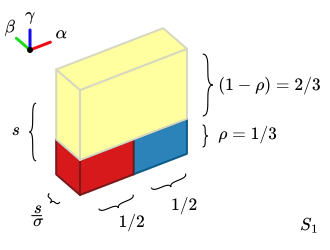
\includegraphics[width=\linewidth]{gilbert3d_eccentric_beta_lt.pdf}
    \caption{ An $S_1$ eccentric subdivision showing the threshold, $\sigma$, used to determine when we should use this split
              and the split point ratio, $\rho$, to reduce the defect for a more harmonious subdivision. }
    \label{fig:eccentric_beta_lt}

  \end{minipage}\hfill
  \begin{minipage}[ht]{0.48\linewidth}

  \centering
  \includegraphics[width=\linewidth]{gilbert3d_eccentric_gamma_lt.pdf}
  \caption{ An $S_1$ eccentric subdivision showing the threshold, $\sigma$, used to determine when we should use this split
            and the split point ratio, $\rho$, to reduce the defect for a more harmonious subdivision. }
  \label{fig:eccentric_gamma_lt}

  \end{minipage}
\end{figure}


When side lengths become too lopsided, an alternate \textit{eccentric} subdivision scheme is chosen to split along
the larger side length.

For each eccentric subdivision, a proportion threshold needs to be chosen to determine when a side
lengths become too lopsided to warrant an alternate subdivision.
Here we motivate the eccentric subdivision constants for the 2D case.

Consider a \textit{defect} function, $\lambda _ 2 : \mathbb{N}^2 \mapsto \mathbb{N}$, that measures the area relative
to what the area would be if it just the minimum side length were taken:

$$
\begin{array}{ll}
  \lambda _ 2 (|\alpha|,|\beta|) = \frac{ |\alpha| \cdot |\beta| }{ \text{min}(|\alpha|,|\beta|)^2 } \\
\end{array}
$$

If there is a disjoint subdivision of a volume $V_0$ to $V_1  = ( V _ {0,0}, V _ {0,1}, \dots, V _ {0,m-1} )$,
($V _ 0  = \cup _ {k} V _ {0,k}$),
define the subdivided volume's \textit{average defect} to be the sum of defects weighted by their proportional volume:

$$
\begin{array}{l}
  \lambda _ {s} ( V _ 1 ) = \sum _ {k} \frac{ \text{Vol}(V _ {0,k}) }{ \text{Vol}( V _ 0 ) } \cdot \lambda _ 2( V _ {0,k} )
\end{array}
$$

The defect gives a coarse idea of how lopsided or \textit{eccentric} a region is.
If the defect is too high, we might want to split the larger sides while keeping the smaller sides the same size.
Reducing the average defect attempts to make each subdivided region more square-like.
When subdivided areas are more square-like, we say that the subdivided regions are more \textit{harmonious}.

If the $\alpha$ side length is significantly longer than the $\beta$ side length,
we want to subdivide the rectangle into two nearly equal regions and recursively find
a Gilbert curve in each region.
We will justify the constant $(3/2)$ as the ratio threshold to split on, using an argument
originally developed by L. Tautenhahn \footnote{ Given to us through personal communication with L. Tautenhahn }.

The defect of a rectangle with side length $|\alpha|$ and $|\beta|$, assuming $|\alpha| > |\beta|$, is $(|\alpha| / |\beta|)$.
After subdivision, if we assume $|\alpha| < 2 |\beta|$, the resulting defect is $2 |\beta| / |\alpha|$.
For a defect reduction, we search for conditions in which the ratio of the resulting defect to the original defect is less than unity,
giving the equation $|\alpha| / |\beta| > \sqrt{2}$.

%$$
%\begin{array}{ll}
%  \lambda_2(|\alpha|, |\beta|) & = |\alpha| \cdot |\beta| / |\beta|^2 \\
%   & = |\alpha| / |\beta|
%\end{array}
%$$
%
%After a subdivision, if we assume $|\alpha| < 2 |\beta|$, the defect is:
%
%$$
%\begin{array}{ll}
%  \lambda_2(|\alpha|/2, |\beta|) & = \frac{|\alpha|}{2} \cdot |\beta| / (\frac{|\alpha|}{2})^2 \\
%   & = 2 |\beta| / |\alpha|
%\end{array}
%$$
%
%We're looking for the condition when there's a defect reduction, so
%
%$$
%\begin{array}{ll}
%    & \lambda_2(|\alpha|/2, |\beta|)  < \lambda_2(|\alpha|, |\beta|) \\
%\to & 2 |\beta| / |\alpha| < |\alpha| / |\beta| \\
%  \to & \sqrt{2} < |\alpha| / |\beta| \\
%\end{array}
%$$

Since $\sqrt{2} \approx 1.4142 < (3/2)$, if we choose $|\alpha| / |\beta| > (3/2)$ we can
be assured a defect reduction.
In the case when $|\alpha| > 2 |\beta|$, it is easy to verify that the defect is always reduced
\footnote{ The ratio of the defects before and after the split is $(1/2)$ }.

Defect reductions for the 3D case can be done, but are more complicated.
The constants for the 3D subdivision in this paper were observed to yield visually pleasing results
without concern for defect optimization.

\section*{Algorithm}


\begin{minipage}[ht]{0.45\linewidth}
\begin{algorithm}[H]
  \caption{ }
  \label{alg:gilbert2d}
  \begin{algorithmic}

    \State \textit{\# $p, \alpha, \beta \in \mathbb{Z}^3$}
    \Function{Gilbert2D}{$p$, $\alpha$, $\beta$}
      \State $\alpha_2, \beta_2  = \text{div}(\alpha, 2), \text{div}(\beta, 2)$
      \If{ $(|\beta| \equiv 1)$ }
        \State \textbf{yield} $p + i \cdot \delta(\alpha)$ \textbf{forall} $i \in |\alpha|$
      \ElsIf{ $(|\alpha| \equiv 1)$ }
        \State \textbf{yield} $p + i \cdot \delta(\alpha)$ \textbf{forall} $i \in |\beta|$
      \ElsIf{ $(2 |\alpha| > 3 |\beta|)$ }
        \If{ $(|\alpha_2| > 2)$ and \\ \hskip4.12em $(|\alpha_2| \bmod{2} \equiv 1)$ }
          \State $\alpha_2 \leftarrow \alpha_2 + \delta(\alpha)$
        \EndIf
        \State \textbf{yield} Gilbert2D($p$, $\alpha_2$, $\beta$)
        \State \textbf{yield} Gilbert2D($p + \alpha_2$, $\alpha - \alpha_2$, $\beta$)
      \Else
        \If{ $(|\beta_2| > 2)$ and \\ \hskip4.12em $(|\beta_2| \bmod{2} \equiv 1)$ }
          \State $\beta_2 \leftarrow \beta_2 + \delta(\beta)$
        \EndIf
        \State \textbf{yield} Gilbert2D($p$, \\ \hskip9.75em $\beta_2$, $\alpha_2$)
        \State \textbf{yield} Gilbert2D($p + \beta_2$, \\ \hskip9.75em $\alpha$, $(\beta - \beta_2)$)
        \State \textbf{yield} Gilbert2D($p + \alpha - \delta(\alpha) + \beta_2 - \delta(\beta)$, \\ \hskip9.75em $\beta_2$, $-(\alpha - \alpha_2)$)
      \EndIf
    \EndFunction

  \end{algorithmic}
\end{algorithm}
\end{minipage}\hfill
\begin{minipage}[ht]{0.45\linewidth}
\begin{algorithm}[H]
  \caption{ }
  \label{alg:gilbert3d}
  \begin{algorithmic}

    \State \textit{\# $p, \alpha, \beta, \gamma \in \mathbb{Z}^3$}
    \Function{Gilbert3D}{$p$, $\alpha$, $\beta$, $\gamma$}

    \State \Return Gilbert2D($p$,$\beta$,$\gamma$) \textbf{if} $(|\alpha| \equiv 1)$
    \State \Return Gilbert2D($p$,$\alpha$,$\gamma$) \textbf{if} $(|\beta| \equiv 1)$
    \State \Return Gilbert2D($p$,$\alpha$,$\beta$) \textbf{if} $(|\gamma| \equiv 1)$

    \State $\alpha_2 \leftarrow \text{div}(\alpha,2) + \Delta(\alpha _ 2, \alpha)$
    \State $\beta_2 \leftarrow \text{div}(\beta,2) + \Delta(\beta _ 2, \beta)$
    \State $\gamma_2 \leftarrow \text{div}(\gamma,2) + \Delta(\gamma _ 2, \gamma)$

    \State \textbf{if }$(2 |\alpha|>3|\beta|) \text{ and } (2|\alpha|>3|\gamma|))$
    \State \hskip1.0em \textbf{yield} Gilbert3D($p$,$\alpha _ 2$,$\beta$,$\gamma$)
    \State \hskip1.0em \textbf{yield} Gilbert3D($p + \alpha _ 2$,$\alpha - \alpha _ 2$,$\beta$,$\gamma$)
    \State \textbf{if }$(3 |\beta| > 4 |\gamma|)$
    \State \hskip1.0em \textbf{yield} Gilbert3D($p$,$\beta _ 2$,$\gamma$,$\alpha _ 2$)
    \State \hskip1.0em \textbf{yield} Gilbert3D($p + \beta _ 2$,$\alpha$,$\beta - \beta _ 2$,$\gamma$)
    \State \hskip1.0em \textbf{yield} Gilbert3D($p + $ \\ \hskip9.75em $(\alpha - \delta(\alpha)) +$ \\ \hskip9.75em $(\beta _ 2 - \delta(\beta))$, \\ \hskip9.75em $-\beta _ 2$,$\gamma$,$-(\alpha - \alpha _ 2)$)
    \State \textbf{if }$(3 |\gamma| > 4 |\beta|)$
    \State \hskip1.0em \textbf{yield} Gilbert3D($p$,$\gamma _ 2$,$\alpha _ 2$,$\beta$)
    \State \hskip1.0em \textbf{yield} Gilbert3D($p + \gamma _ 2$,$\alpha$, $\beta$, $\gamma - \gamma _ 2$)
    \State \hskip1.0em \textbf{yield} Gilbert3D($p +$ \\ \hskip9.75em $(\alpha - \delta(\alpha))$ \\ \hskip9.75em $(\gamma2 - \delta(\gamma))$, \\ \hskip9.5em $-\gamma _ 2$,$-(\alpha-\alpha _ 2)$, $\beta$)

    \State
    \State \textbf{else }$(3 |\beta| > 4 |\gamma|)$
    \State \hskip1.0em \textbf{yield} Gilbert3D($p$,$\beta _ 2$,$\gamma _ 2$,$\alpha _ 2$)
    \State \hskip1.0em \textbf{yield} Gilbert3D($p + \beta _ 2$,$\gamma$,$\alpha _ 2$,$\beta _ 2$)
    \State \hskip1.0em \textbf{yield} Gilbert3D($p +$ \\ \hskip9.75em $(\beta _ 2 - \delta(\beta)) +$ \\ \hskip9.75em $(\gamma - \delta(\gamma))$, \\ \hskip9.5em $\alpha$,$-\beta_2$,$-(\gamma-\gamma_2)$)
    \State \hskip1.0em \textbf{yield} Gilbert3D($p +$ \\ \hskip9.75em $(\alpha _ 2 - \delta(\alpha)) +$ \\ \hskip9.75em $\beta _ 2 (\gamma - \delta(\gamma))$, \\ \hskip9.5em $-\gamma$,$-(\alpha - \alpha_2)$,$(\beta-\beta_2)$)
    \State \hskip1.0em \textbf{yield} Gilbert3D($p +$ \\ \hskip9.75em $(\alpha - \delta(\alpha)) +$ \\ \hskip9.75em $(\beta _ 2 - \delta(\beta))$, \\ \hskip9.5em $-\beta _ 2$,$-\gamma _ 2$,$-(\alpha - \alpha_2)$)

    \EndFunction

  \end{algorithmic}
\end{algorithm}
\end{minipage}


Algorithm \ref{alg:gilbert2d} shows the pseudo-code for computing the 2D Gilbert curve.
Note that $\alpha$ and $\beta$ are taken to be vectors in 3D, where the third dimension
can be ignored if a purely 2D curve is desired.
The generalization to 3D allows the Gilbert2D function to be used unaltered when the
3D Gilbert curve needs to trace out in-plane sub-curves.

Algorithm \ref{alg:gilbert2d} assumes standard Euclidean two norm ($|v| = \sqrt{v_0^2 + v_1^2 + v_2^2}$)
and abuses notation by allowing scalar to vector multiplication ($i \in \mathbb{Z}, v \in \mathbb{Z}^3, i \cdot v \to ( i \cdot v_0, i \cdot v_1, i \cdot v_2 )$).
where the context is clear.

The $\delta(\cdot)$ function returns one of the six directional vectors indicating which of
the major signed axis aligned directions the input vector points to ($(\pm1,0,0), (0,\pm1,0),(0,0,\pm1)$).
To make things more concise, a convenience function is used,
$(\Delta( \rho_2,\rho ) \overset{\mathrm{def}}{=} \delta(\rho) \textbf{ if } |\rho _ 2| \equiv 1 \bmod{2} \text{ and } |\rho| > 2)$,
that prefers even lengths in the non-degenerate case.


\section*{Conclusion and Future Directions}

The Gilbert curve presented in this paper provides one intepretation for a generalized Hilbert
curve in 2D and 3D to arbitrary side lengths.
Generaliing a Hilbert space filling curve to arbitrary side lengths is not a well posed problem
and is open to interpretation, and the solution presented here is one such adaptation.

When desinging an algorithm to generalize the Hilbert curve, four features that might be desirable are:

\begin{table}[h]
  \centering
  \begin{tabular}[t]{l|l}
    \textit{Hilbert-esque} & Reduces to a Hilbert curve when side lengths are equal and are exact powers of two \\
    \textit{Stabilty} & Curve realizations converge as the cuboid side lengths increase proportionally \\
    \textit{Harmony} & Realizations use eccentric splits to reduce the \textit{defect} \\
    \textit{Notch-Limited} & Curve realizations are notch free unless a single notch is necessary \\
  \end{tabular}
\end{table}

The 2D Gilbert curve presented here has all of these properties while the 3D Gilbert curve lacks harmony and the notch-limited feature.

Future work could focus on creating 3D Gilbert curve that has all of these features, perhaps by relaxing strict endpoint requirements
at the cuboid corners.
Some other natural ideas are to extend the concepts above to other space filling curves or ciruits,
or, more generally, to try and create an arbitrary space filling curve in a cuboid region with arbitrary endpoints.

A libre/free implementation for the Gilbert curve in 2D and 3D has been developed and can be downloaded from its
repository \footnote{ \label{gilbert-url} \url{https://github.com/jakubcerveny/gilbert} }.




%\bibliographystyle{unsrtnat}
%\bibliography{06-References}


{\setlength{\baselineskip}{13pt} % tighten line spacing for bibliography
\raggedright        % no right justification for References
\begin{thebibliography}{99}


  \bibitem{lutanho2003} L. Tautenhahn. ``Draw a space-filling curve of arbitrary size.'' 2003. \url{https://lutanho.net/pic2html/draw_sfc.html}.


%
%\bibitem{Chang}
%W. Chang. \LaTeX\ \textit{Cheat Sheet}. 2014. \url{http://wch.github.io/latexsheet/}.
%
%\bibitem{EJCx}
%M.\ Chladn\'y and M.\ \v Skoviera. ``Factorisation of Snarks.'' \textit{Electronic Journal
%of Combinatorics}, vol.~17, no.~1, R32, 2010.
%\url{http://www.combinatorics.org/Volume_17/PDF/v17i1r32.pdf}.
%
%\bibitem{Coxeter} H.\ S.\ M.\ Coxeter. ``The Non-Euclidean Symmetry of Escher's Picture
%Circle Limit III.'' \textit{Leonardo}, vol.~12, no.~1, 1979, pp.~19--25.
%
%\bibitem{easychair} EasyChair. Log in page. \url{https://easychair.org/account/signin.cgi}.
%
%\bibitem{Gratzer} G.\ Gr\"atzer. \textit{More Math Into} \LaTeX, 4th ed. Springer, 2007.
%
%\bibitem{Sequin2016} C.\ H.\ S\'equin. ``From Klein Bottles to Modular Super-Bottles.''
%\textit{Bridges Conference Proceedings}, Jyv\"askyl\"a, Finland, Aug. 9--13,
%2016, pp.~41--48. \url{http://archive.bridgesmathart.org/2016/bridges2016-41.html}.
%

\end{thebibliography}
} % end setlength, raggedright


\begin{figure}[ht]
  \centering
  \includegraphics[width=\linewidth]{gilbert_bd50x10.pdf}
  \label{fig:footerGilbert}
\end{figure}

%  \caption{ Illustrative examples of Hamiltonian paths height/width that are even/even, even/odd and odd/odd, respectively, when starting from the lower left hand corner }



%\appendix
%
%\clearpage

\section{Appendix}


\subsection{Defect} \label{appendix:defect}

Call the \textit{defect} a function $\lambda _ d : \mathbb{N}^d \mapsto \mathbb{N}$:

$$
\begin{array}{l}
\lambda _ 2 (|\alpha|,|\beta|) = \frac{ |\alpha| \cdot |\beta| }{ \text{min}(|\alpha|,|\beta|)^2 } \\
\lambda _ 3 (|\alpha|,|\beta|,|\gamma|) = \frac{ |\alpha| \cdot |\beta| \cdot |\gamma| }{ \text{min}(|\alpha|,|\beta|,|\gamma|)^3 }
\end{array}
$$

If there is a disjoint subdivision of a volume $V_0$ to $V_1  = ( V _ {0,0}, V _ {0,1}, \dots, V _ {0,m-1} )$,
$V _ 0  = \cup _ {k} V _ {0,k}$,
define the \textit{average defect} of the subdivided volume to be:

$$
\begin{array}{l}
  \lambda _ {s} ( V _ 1 ) = \sum _ {k} \frac{ \text{Vol}(V _ {0,k}) }{ \text{Vol}( V _ 0 ) } \cdot \lambda( V _ {0,k} )
\end{array}
$$

This weights the defect of each subdivided cuboid by its proportional volume.

The defect gives us a coarse idea of how lopsided or \textit{eccentric} a cuboid region is.
If the defect is too high, we might want to split the larger sides while keeping the smaller sides the same size.

\subsection{2D Eccentric Split Threshold}

For the 2D Gilbert curve,
if the $\alpha$ side length is significantly longer than the $\beta$ side length,
we want to subdivide the rectangle into two nearly equal regions and recursively find
a Gilbert curve in each region.
We will justify the constant $(3/2)$ as the ratio threshold to split on using an argument
given by L. Tautenhahn \footnote{ through personal communication }.
That is, when $(|\alpha|/|\beta| > 3/2)$, we split the rectangle into roughly equal parts.

The defect of a rectangle of side length $|\alpha|$ and $|\beta|$ is, with $|\alpha| > |\beta|$:

$$
\begin{array}{ll}
  \lambda_2(|\alpha|, |\beta|) & = |\alpha| \cdot |\beta| / |\beta|^2 \\
   & = |\alpha| / |\beta|
\end{array}
$$

After a subdivision, if we assume $|\alpha| < 2 |\beta|$, the defect is:

$$
\begin{array}{ll}
  \lambda_2(|\alpha|/2, |\beta|) & = \frac{|\alpha|}{2} \cdot |\beta| / (\frac{|\alpha|}{2})^2 \\
   & = 2 |\beta| / |\alpha|
\end{array}
$$

We're looking for the condition when there's a defect reduction, so

$$
\begin{array}{ll}
    & \lambda_2(|\alpha|/2, |\beta|)  < \lambda_2(|\alpha|, |\beta|) \\
\to & 2 |\beta| / |\alpha| < |\alpha| / |\beta| \\
  \to & \sqrt{2} < |\alpha| / |\beta| \\
\end{array}
$$

Since $\sqrt{2} \approx 1.4142 < (3/2)$, if we choose $|\alpha| / |\beta| > (3/2)$ we can
be assured a defect reduction.


\subsection{3D Eccentric Split Threshold}

Calculations in this section will justify what threshold value to pick of when to choose a 3D
eccentric split over a J-split.
Our concern is to find a simple ratio of when each of $\alpha$, $\beta$ or $\gamma$ are considered
"small enough" or "large enough", relative to the other dimensions, to split on.

An enumeration of what conditions lead to an eccentric split are as follows:

$$
\begin{array}{ll}
  (1) & |\alpha| >> |\beta| \sim |\gamma| \\
  (2) & |\beta| >> |\alpha| \sim |\gamma| \\
  (3) & |\gamma| >> |\alpha| \sim |\beta| \\
  (4) & |\beta| << |\alpha| \sim |\gamma| \\
  (5) & |\alpha| << |\beta| \sim |\gamma| \\
  (6) & |\gamma| << |\alpha| \sim |\beta| \\
\end{array}
$$

A representation of the eccentric splits are enumerated in Figure \ref{fig:gilbert3DEccentricCase}.
The eccentric $S$-split split differs from the $J$-split as it's only partitioning the cuboid along
one or two dimensions instead of three.

For each of the six cases, we want to know what relative difference in sizes should be used
to determine when an eccentric split should be used and how to subdivide the cuboids so as to make
the resulting subdivided cuboids more cube-like.

Specifically, we want to find the ratio, $\sigma$, of when one dimension is proportionally larger or smaller,
respectively, than the others.
Further, we choose the ratio, $\rho$, of where to choose the split point of subdivision.
For simplicity, we might want to subdivide at the half way point ($\rho = \frac{1}{2}$) but as we
will see, this might give lopsided sub-cuboid regions and using a better split point is desirable.

In what follows, our goal is to choose a subdivision that will reduce the average defect.
We assume that the start and end of the path lie in the $\alpha$ dimension.

Since the start and end path lie on the $\alpha$ dimension, we are forced to split in the $\alpha$ axis
to subdivide the cuboid.
In what follows, we always commit to splitting the $\alpha$ cuboid region by half, with a potentially
additional step to coerce the $A$ volume to a desired parity.

%%%%
%%%%
%%%%

\subsection{$|\alpha| >> |\beta| \sim |\gamma|$}

\begin{itemize}
  \item Shape template: $S_0$
  \item $\sigma = \frac{5}{3}$
  \item $\rho = \text{n/a}$
\end{itemize}


When $|\alpha|$ is much larger than $|\beta|$ or $|\gamma|$,
we split into two sub-cuboids along the $\alpha$ axis,
which we represent as an $S_0$ split.
As stated above, we pick the midway point for $\alpha$.
What's left is to decide how eccentric the cuboid should be to make the $S_0$ split.

Take $\sigma > 1$ and $s = \text{min}(|\beta|,|\gamma|)$, $\sigma s = |\alpha|$.
The defect of the original volume is:

$$
\begin{array}{ll}
  \lambda(|\alpha|,|\beta|,|\gamma|)  & = \frac{ |\alpha| \cdot |\beta| \cdot |\gamma| }{ \text{min}(|\alpha|,|\beta|,|\gamma|) } \\
                  & = \frac{ \sigma s \cdot s \cdot s }{ \text{min}(\sigma s,s,s) } \\
                  & = \sigma \\
\end{array}
$$

If $|\alpha| > 2 |\beta| = 2s$, then $\text{min}(\frac{|\alpha|}{2},|\beta|,|\gamma|) = s$ and we have an average defect $\lambda_s(V_1) = \frac{\sigma}{2}$.
Intuitively, we reduce the defect by splitting a long horizontal column into two parts, each of which is more cube like,
making it more cube-like on average.

We can get a better ratio of when to split by asking what the maximum value of $|\alpha| = \sigma s$ is when there is still an average defect reduction.
In this case, we restrict $|\alpha| < 2 |\beta|$, with $\text{min}(\frac{|\alpha|}{2},|\beta|,|\gamma|) = \frac{|\alpha|}{2}$,
the average defect becomes:

$$
\begin{array}{ll}
  \lambda_s(V_1) & = 2 (\frac{1}{2}) \frac{ \frac{\sigma}{2} \cdot s^3 }{ (\frac{\sigma}{2} s)^3 } \\
   & = \frac{4}{\sigma^2}
\end{array}
$$

We want to reduce the average defect relative to the original defect, so:

$$
\begin{array}{ll}
  & \lambda_s (V_1) < \lambda(V_0) \\
  \to & \frac{4}{\sigma^2} < \sigma \\
  \to & 4^{\frac{1}{3}} < \sigma \\ 
  \to & 4^{\frac{1}{3}} = 1.58740\dots < \sigma < \frac{5}{3} \\
\end{array}
$$

For any $\sigma > 4^{\frac{1}{3}}$, we know the average defect will be reduced.
For algorithmic simplicity, we've chosen the simple fraction $\frac{5}{3}$ (as $\frac{5}{3} > 4^{\frac{1}{3}}$)
for the eccentric $S_0$ split ratio.

%%%%
%%%%
%%%%

\subsection{$|\gamma| >> |\alpha| \sim |\beta|$ or $|\beta| << |\alpha| \sim |\gamma|$}


\begin{figure}[h]
  \centering
  \includegraphics[width=\linewidth]{gilbert3d_eccentric_appendix_s1.pdf}
  \caption{ An $S_1$ eccentric subdivision showing the threshold, $\sigma$, used to determine when we should use this split
            and the split point ratio, $\rho$, to reduce the defect for a more harmonious subdivision. }
  \label{fig:eccentric_s1}
\end{figure}



\begin{itemize}
  \item Shape template: $S_1$
  \item $\sigma = \frac{3}{2}$
  \item $\rho = \frac{1}{3}$
\end{itemize}

Here, we are trying to validate two parameters, $\sigma$ and $\rho$.
$\sigma$ is the ratio of when $|\gamma|$ (resp. $|\beta|$)
is larger (resp. smaller) to the minimum (resp. maximum) of the remaining side lengths as the threshold to trigger an $S_1$
template split.
$\rho$ is the proportion along the $\gamma$ (resp. $\beta$) direction of where to choose the $\gamma$ direction split.
The $S_1$ shape template has three subdivided cuboids, which we call $A$, $B$ and $C$, ordered by
the path traversal through the cuboids.

We will show that there is an average defect reduction when choosing $\sigma = \frac{3}{2}$ and
$\rho = \frac{1}{3}$.
If we take $s = \text{min}(|\alpha|, |\beta|)$ and $|\gamma| = \sigma s$, then the defect of the original volume is:

$$
\lambda(V_0) = \sigma
$$

From our choice of $\sigma$ and $\rho$, $\text{min}( \sigma \rho s, \frac{s}{2} ) = \frac{s}{2}$,
implying the minimum side length for $A$ and $C$ is $\frac{s}{2}$ and the minimum side length of $B$
is $\text{min}( \sigma (1-\rho) s, s) = s$.
From this, we can calculate the average defect of the subdivided cuboid:

$$
\begin{array}{ll}
  \lambda_s (V_1) & = 2 \cdot (\frac{1}{2}) \rho [ \frac{ \rho \sigma s \cdot \frac{s}{2} \cdot s }{ (\frac{s}{2})^3 } ] \\
        & + (1-\rho) [ \frac{ (1-\rho) \sigma s \cdot s \cdot s }{s^3} ] \\
   & = 4 \sigma \rho^2 + \sigma (1-\rho)^2 \\
  & = 4 \sigma \rho^2 + \sigma (1-\rho)^2 \\
  & = \frac{8}{9} \sigma = \frac{4}{3} < \frac{3}{2} \\
  \to & \lambda_s(V_1) < \lambda(V_0)
\end{array}
$$

Showing there is an average defect reduction.

%%%%
%%%%
%%%%


\subsection{$|\beta| >> |\alpha| \sim |\gamma|$ or $|\alpha| << |\beta| \sim |\gamma|$}

\begin{figure}[h]
  \centering
  \includegraphics[width=\linewidth]{gilbert3d_eccentric_appendix_s2.pdf}
  \caption{ An $S_2$ eccentric subdivision showing the threshold, $\sigma$, used to determine when we should use this split
            and the split point ratio, $\rho$, to reduce the defect for a more harmonious subdivision. }
  \label{fig:eccentric_s2}
\end{figure}

\begin{itemize}
  \item Shape template: $S_2$
  \item $\sigma = \frac{3}{2}$
  \item $\rho = \frac{1}{3}$
\end{itemize}

As with the previous case, we are trying to validate two parameters, $\sigma$, the amount
of eccentricity of one side length relative to the others, and $\rho$, where to subdivide the
cuboid along the $\beta$ axis.

Choosing $\sigma = \frac{3}{2}$ implies that the defect of the original volume is $\lambda(V_0) = \sigma = \frac{3}{2}$.
Further, $\text{min}( \sigma \rho s, \frac{s}{2} ) = \frac{s}{2}$, implying the $A$ and $C$ volumes
have minimum side length of $\frac{s}{2}$ and $\text{min}( (1-\rho) \sigma s, s) = s$, implying the
minimum side length of volume $C$ is $s$.

This allows us to calculate the average defect of the subdivided cuboid using an $S_2$ shape template:

$$
\begin{array}{ll}
  \lambda_s (V_1) & = 2 (\frac{1}{2}) \rho [ \frac{ \rho \sigma s \cdot \frac{s}{2} \cdot s }{(\frac{s}{2})^3} ] \\
  & + (1-\rho) \cdot [ \frac{ (1-\rho) \sigma s \cdot s \cdot s }{s^3} ] \\
  & = 4 \sigma \rho^2 + \sigma (1-\rho)^2 \\
  & = \frac{8}{9} \sigma = \frac{4}{3} < \frac{3}{2} \\
  \to & \lambda_s(V_1) < \lambda(V_0) \\
\end{array}
$$



%
\clearpage

\section{Auxiliary Algorithms and Procedures} \label{ProcedureAppendix}

\subsection{Auxiliary Functions} \label{AuxiliaryFunctions}

\floatname{algorithm}{Auxiliary Functions}
\begin{algorithm}
  \caption{\hskip0.5em}
  \label{alg:delta}
  \begin{algorithmic}

    \State
    \State \textit{\# integral sign function}
    \Function{$\text{sgn}$}{$w \in \mathbb{Z}$}
      %\State $(w < 0) ? (-1) : ((w > 0) ? 1 : 0)$
      \State \textbf{if} $(w < 0)$ \Return $-1$
      \State \textbf{if} $(w > 0)$ \Return $1$
      \State \Return 0
    \EndFunction

    \State
    \State \textit{\# vector integer round down divide}
    \Function{$\text{div}$}{$v \in \mathbb{Z}^3$, $q \in \mathbb{Z}$ }
      \State $u_0 = \text{sgn}(v_0) \lfloor | \frac{v_0}{q} | \rfloor$
      \State $u_1 = \text{sgn}(v_1) \lfloor | \frac{v_1}{q} | \rfloor$
      \State $u_2 = \text{sgn}(v_2) \lfloor | \frac{v_2}{q} | \rfloor$
      \State \Return $(u_0, u_1, u_2)$
    \EndFunction

    \State
    \State \textit{\# directional vector}
    \Function{$\delta$}{$v \in \mathbb{Z}^3$}
      \State \Return $( \text{sgn}(v_0), \text{sgn}(v_1), \text{sgn}(v_2) )$
    \EndFunction

    \State
    \State \textit{\# Test if $q$ in directional volume with origin $p$}
    \Function{inBounds}{$q, p, \alpha, \beta, \gamma \in \mathbb{Z}^3$}
      \State $v \leftarrow \alpha + \beta + \gamma$
      \For{$i \leftarrow 0$ \textbf{to} $2$}
        \State \textbf{return} \textit{false} \textbf{if} $(\text{sgn}(v_i) \cdot (q_i - p_i) < 0)$
        \State \textbf{return} \textit{false} \textbf{if} $(\text{sgn}(v_i) \cdot (q_i - p_i - v_i) \ge 0)$
      \EndFor
      \State \Return \textit{true}
    \EndFunction

    \State
    \State \textit{\# base case}
    \Function{Hilbert2x2x2}{$p$, $\alpha$, $\beta$, $\gamma$}
      \State \textbf{yield} $p$
      \State \textbf{yield} $p + \delta(\beta)$
      \State \textbf{yield} $p + \delta(\beta) + \delta(\gamma)$
      \State \textbf{yield} $p + \delta(\gamma)$
      \State \textbf{yield} $p + \delta(\alpha) + \delta(\gamma)$
      \State \textbf{yield} $p + \delta(\alpha) + \delta(\beta) + \delta(\gamma)$
      \State \textbf{yield} $p + \delta(\alpha) + \delta(\beta)$
      \State \textbf{yield} $p + \delta(\alpha)$
    \EndFunction

  \end{algorithmic}
\end{algorithm}
\floatname{algorithm}{Algorithm}

\clearpage

\subsection{Gilbert3D S-Split Functions} \label{SSplitFunctions}

\floatname{algorithm}{Procedure}
\begin{algorithm}
  \caption{ \hskip0.5em $S_0$-Split function (eccentric split) }
  \label{alg:procS0}
  \begin{algorithmic}
    \State
    \State \textit{\# split halfway on $\alpha$ }
    \Function{$S_0$}{$p$, $\alpha$, $\beta$, $\gamma$}
      \State $\alpha_2 \leftarrow \text{div}(\alpha, 2)$
      \If{ $(|\alpha| > 2)$ and $((|\alpha_2| \bmod{2}) \equiv 1)$ }
        \State $\alpha_2 \leftarrow \alpha_2 + \delta(\alpha)$
      \EndIf
      \State
      \State \textbf{yield} Gilbert3D($p$, \\ \hskip8.25em $\alpha_{2}$, $\beta$, $\gamma$ )
      \State
      \State \textbf{yield} Gilbert3D($p + \alpha_{2}$, \\ \hskip8.25em $(\alpha - \alpha_{2})$, $\beta$, $\gamma$ )
    \EndFunction
  \end{algorithmic}
\end{algorithm}
\floatname{algorithm}{Algorithm}


\floatname{algorithm}{Procedure}
\begin{algorithm}
  \caption{ \hskip0.5em $S_1$-Split function (eccentric split) }
  \label{alg:procS1}
  \begin{algorithmic}
    \State
    \State \textit{\# split $\frac{1}{3}$ on $\gamma$ and halfway on $\alpha$ }
    \Function{$S_1$}{$p$, $\alpha$, $\beta$, $\gamma$}
      \State $\alpha_2, \gamma_3 \leftarrow \text{div}(\alpha, 2), \text{div}(\gamma, 3)$
      \If{ $(|\alpha| > 2)$ and $((|\alpha_2| \bmod{2}) \equiv 1)$ }
        \State $\alpha_2 \leftarrow \alpha_2 + \delta(\alpha)$
      \EndIf
      \If{ $(|\gamma| > 2)$ and $((|\gamma_3| \bmod{2}) \equiv 1)$ }
        \State $\gamma_3 \leftarrow \gamma_3 + \delta(\gamma)$
      \EndIf
      \State
      \State \textbf{yield} Gilbert3D($p$, \\ \hskip8.25em $\gamma_3$, $\alpha_2$, $\beta$)
      \State
      \State \textbf{yield} Gilbert3D($p + \gamma_3$, \\ \hskip8.25em $\alpha$, $\beta$, $(\gamma - \gamma_3)$)
      \State
      \State \textbf{yield} Gilbert3D($p + \alpha - \delta(\alpha) + \gamma_{3} - \delta(\gamma)$, \\ \hskip8.25em $\gamma_3$, $(\alpha - \alpha_2)$, $\beta$)
    \EndFunction
  \end{algorithmic}
\end{algorithm}
\floatname{algorithm}{Algorithm}


\floatname{algorithm}{Procedure}
\begin{algorithm}
  \caption{ \hskip0.5em $S_2$-Split function (eccentric split) }
  \label{alg:procS2}
  \begin{algorithmic}
    \State
    \State \textit{\# split $\frac{1}{3}$ on $\beta$ and halfway on $\alpha$ }
    \Function{$S_2$}{$p$, $\alpha$, $\beta$, $\gamma$}
      \State $\alpha_2, \beta_3 \leftarrow \text{div}(\alpha, 2), \text{div}(\beta, 3)$
      \If{ $(|\alpha| > 2)$ and $((|\alpha_2| \bmod{2}) \equiv 1)$ }
        \State $\alpha_2 \leftarrow \alpha_2 + \delta(\alpha)$
      \EndIf
      \If{ $(|\beta| > 2)$ and $((|\beta_3| \bmod{2}) \equiv 1)$ }
        \State $\beta_3 \leftarrow \beta_3 + \delta(\beta)$
      \EndIf
      \State
      \State \textbf{yield} Gilbert3D($p$, \\ \hskip8.25em $\beta_{3}$, $\gamma$, $\alpha_2$ )
      \State
      \State \textbf{yield} Gilbert3D($p + \beta_{3}$, \\ \hskip8.25em $\alpha$, $(\beta - \beta_{3})$, $\gamma$ )
      \State
      \State \textbf{yield} Gilbert3D($p + \alpha - \delta(\alpha) + \beta_{3} - \delta(\beta)$, \\ \hskip8.25em $-\beta_{3}$, $\gamma$, $-\alpha$)
    \EndFunction
  \end{algorithmic}
\end{algorithm}
\floatname{algorithm}{Algorithm}

\clearpage

\subsection{Gilbert3D J-Split Functions} \label{JSplitFunctions}

\floatname{algorithm}{Procedure}
\begin{algorithm}
  \caption{ \hskip0.5em $J_0$-Split function }
  \label{alg:procJ0}
  \begin{algorithmic}
    \State
    \State \textit{\# $|\gamma|$ even }
    \Function{$J_0$}{$p$, $\alpha$, $\beta$, $\gamma$}
      \State
      \State $\alpha_2, \beta_2, \gamma_2 \leftarrow \text{div}(\alpha, 2), \text{div}(\beta, 2), \text{div}(\gamma, 2)$
      \State
      \State \textit{\# prefer initial block even}
      \State $\alpha_2 = \alpha_2 + \delta(\alpha)$ \textbf{if} $(| \alpha | > 2)$and$(| \alpha_2 | \bmod{2} \equiv 1)$
      \State $\beta_2 = \beta_2 + \delta(\beta)$ \textbf{if} $(| \beta | > 2)$and$(|\beta_2| \bmod{2} \equiv 1)$
      \State $\gamma_2 = \gamma_2 + \delta(\gamma)$ \textbf{if} $(| \gamma | > 2)$and$(|\gamma_2| \bmod{2} \equiv 1)$
      \State
      \State \textbf{yield} Gilbert3D($p$, \\ \hskip8.25em $\beta_2$, $\gamma_2$, $\alpha_2$)
      \State
      \State \textbf{yield} Gilbert3D($p+\beta_2$, \\ \hskip8.25em $\gamma$, $\alpha_2$, $\beta - \beta_2$)
      \State
      \State \textbf{yield} Gilbert3D($p + \beta_2 - \delta(\beta) + \gamma - \delta(\gamma)$, \\ \hskip8.25em $\alpha$, $-\beta_2$, $-(\gamma - \gamma_2)$)
      \State
      \State \textbf{yield} Gilbert3D($p + \alpha - \delta(\alpha) + \beta_2 + \gamma - \delta(\gamma)$, \\ \hskip8.25em $-\gamma$, $-(\alpha - \alpha_2)$, $(\beta - \beta_2)$)
      \State
      \State \textbf{yield} Gilbert3D($p + \alpha - \delta(\alpha) + \beta_2 - \delta(\beta)$, \\ \hskip8.25em $-\beta_2$, $\gamma_2$, $-(\alpha - \alpha_2)$)
    \EndFunction
  \end{algorithmic}
\end{algorithm}
\floatname{algorithm}{Algorithm}



\floatname{algorithm}{Procedure}
\begin{algorithm}
  \caption{ \hskip0.5em $J_1$-Split function }
  \label{alg:procJ2}
  \begin{algorithmic}
    \State
    \State \textit{\# $|\gamma|$ odd, one of $|\alpha|$ or $|\beta|$ even }
    \Function{$J_1$}{$p$, $\alpha$, $\beta$, $\gamma$}
      \State
      \State $\alpha_2, \beta_2, \gamma_2 \leftarrow \text{div}(\alpha, 2), \text{div}(\beta, 2), \text{div}(\gamma, 2)$
      \State
      \State \textit{\# prefer $\beta_2$, $\gamma_2$ even but force $\alpha_2$ odd }
      \State $\alpha_2=\alpha_2+\delta(\alpha)$ \textbf{if} $(|\alpha| > 2)$and$(|\alpha_2| \bmod{2} \equiv 0)$
      \State $\beta_2=\beta_2+\delta(\beta)$ \textbf{if} $(|\beta| > 2)$and$(|\beta_2| \bmod{2} \equiv 1)$
      \State $\gamma_2=\gamma_2+\delta(\gamma)$ \textbf{if} $(|\gamma| > 2)$and$(|\gamma_2| \bmod{2} \equiv 1)$
      \State
      \State \textbf{yield} Gilbert3D($p$, \\ \hskip8.25em $\gamma_2$, $\alpha_2$, $\beta_2$)
      \State
      \State \textbf{yield} Gilbert3D($p+\gamma_2$, \\ \hskip8.25em $\beta$, $\gamma - \gamma_2$, $\alpha_2$)
      \State
      \State \textbf{yield} Gilbert3D($p+\gamma_2 - \delta(\gamma) + \beta - \delta(\beta)$, \\ \hskip8.25em $\alpha$, $-(\beta - \beta_2)$, $-\gamma_2$)
      \State
      \State \textbf{yield} Gilbert3D($p+\alpha - \delta(\alpha) + \beta - \delta(\beta) + \gamma_2$, \\ \hskip8.25em $\beta$, $\gamma - \gamma_2$, $-(\alpha - \alpha_2)$)
      \State
      \State \textbf{yield} Gilbert3D($p+\alpha - \delta(\alpha) + \gamma_2 - \delta(\gamma)$, \\ \hskip8.25em $-\gamma_2$, $-(\alpha - \alpha_2)$, $\beta_2$)
    \EndFunction
  \end{algorithmic}
\end{algorithm}
\floatname{algorithm}{Algorithm}


\floatname{algorithm}{Procedure}
\begin{algorithm}
  \caption{ \hskip0.5em $J_2$-Split function }
  \label{alg:procJ2}
  \begin{algorithmic}
    \State
    \State \textit{\# $|\alpha|, |\beta|, |\gamma|$ odd }
    \Function{$J_2$}{$p$, $\alpha$, $\beta$, $\gamma$}
      \State
      \State $\alpha_2, \beta_2, \gamma_2 \leftarrow \text{div}(\alpha, 2), \text{div}(\beta, 2), \text{div}(\gamma, 2)$
      \State
      \State \textit{\# prefer $\beta_2$, $\gamma_2$ even but force $\alpha_2$ odd }
      \State $\alpha_2=\alpha_2+\delta(\alpha)$ \textbf{if} $(|\alpha| > 2)$and$(|\alpha_2| \bmod{2} \equiv 0)$
      \State $\beta_2=\beta_2+\delta(\beta)$ \textbf{if} $(|\beta| > 2)$and$(|\beta_2| \bmod{2} \equiv 1)$
      \State $\gamma_2=\gamma_2+\delta(\gamma)$ \textbf{if} $(|\gamma| > 2)$and$(|\gamma_2| \bmod{2} \equiv 1)$
      \State
      \State \textbf{yield} Gilbert3D($p$, \\ \hskip8.25em $\beta_2$, $\gamma$, $\alpha_2$)
      \State
      \State \textbf{yield} Gilbert3D($p+\beta_2$, \\ \hskip8.25em $\gamma_2$, $\alpha$, $(\beta - \beta_2)$)
      \State
      \State \textbf{yield} Gilbert3D($p+\beta_2 + \gamma_2$, \\ \hskip8.25em $\alpha$, $(\beta - \beta_2)$, $(\gamma - \gamma_2)$)
      \State
      \State \textbf{yield} Gilbert3D($p + \alpha - \delta(\alpha) + \beta_2 - \delta(\beta) + \gamma_2$, \\ \hskip8.25em $-\beta_2$, $(\gamma- \gamma_2)$, $-(\alpha - \delta(\alpha))$) 
      \State
      \State \textbf{yield} Gilbert3D($p + \alpha - \delta(\alpha) + \gamma_2 - \delta(\gamma)$, \\ \hskip8.25em $-\gamma_2$, $-(\alpha - \alpha_2)$, $\beta_2$)
    \EndFunction
  \end{algorithmic}
\end{algorithm}
\floatname{algorithm}{Algorithm}


\clearpage

\subsection{Gilbert2D Lookup Functions}

\floatname{algorithm}{Algorithm}
\begin{algorithm}[tbh]
  \caption{\hskip0.5em 2D Generalized Hilbert Index to Position Lookup Function (Gilbert2D\_d2xyz) }
  \label{alg:gilbert2d_d2xyz}
  \begin{algorithmic}

    \State \textit{\# $d_{\text{dst}}, d_{\text{cur}} \in \mathbb{Z}, p, \alpha, \beta \in \mathbb{Z}^3$}
    \Function{Gilbert2D\_d2xyz}{$d_{\text{dst}}$, $d_{\text{cur}}$, $p$, $\alpha$, $\beta$}
      \State
      \State $\alpha_2, \beta_2  = \text{div}(\alpha, 2), \text{div}(\beta, 2)$

      \State
      \If{ $(|\beta| \equiv 1)$ }
        \State \Return $p + (d_{\text{dst}} - d_{\text{cur}}) \cdot \delta(\alpha)$
      \ElsIf{ $(|\alpha| \equiv 1)$ }
        \State \Return $p + (d_{\text{dst}} - d_{\text{cur}}) \cdot \delta(\beta)$

        \State
      \ElsIf{ $(2 |\alpha| > 3 |\beta|)$ }
        \If{ $(|\alpha_2| > 2)$ and $(|\alpha_2| \bmod{2} \equiv 1)$ }
          \State $\alpha_2 \leftarrow \alpha_2 + \delta(\alpha)$
        \EndIf
        \State
        \State $d_{\text{nxt}} \leftarrow d_{\text{cur}} + |\alpha_2| \cdot |\beta|$
        \If{ $d_{\text{cur}} \le d_{\text{dst}} < d_{\text{nxt}}$ }
          \State \Return Gilbert2D\_d2xyz($d_{\text{dst}}$, $d_{\text{cur}}$, \\ \hskip15.0em $p$, \\ \hskip15.0em $\alpha_2$, $\beta$)
        \EndIf
        \State

        \State $d_{\text{cur}} \leftarrow d_{\text{nxt}}$
        \State \Return Gilbert2D\_d2xyz($d_{\text{dst}}$, $d_{\text{cur}}$, \\ \hskip13.5em $p + \alpha_2$, \\ \hskip13.5em $\alpha - \alpha_2$, $\beta$)

        \State
      \EndIf
      \State

      \If{ $(|\beta_2| > 2)$ and $(|\beta_2| \bmod{2} \equiv 1)$ }
        \State $\beta_2 \leftarrow \beta_2 + \delta(\beta)$
      \EndIf
      \State
      \State $d_{\text{nxt}} \leftarrow d_{\text{cur}} + |\beta_2| \cdot |\alpha_2|$
      \If{ $d_{\text{cur}} \le d_{\text{dst}} < d_{\text{nxt}}$ }
        \State \Return Gilbert2D\_d2xyz($d_{\text{dst}}$, $d_{\text{cur}}$, \\ \hskip13.5em $p$, \\ \hskip13.5em $\beta_2$, $\alpha_2$)
      \EndIf
      \State $d_{\text{cur}} \leftarrow d_{\text{nxt}}$
      \State

      \State $d_{\text{nxt}} \leftarrow d_{\text{cur}} + |\alpha| \cdot |\beta-\beta_2|$
      \If{ $d_{\text{cur}} \le d_{\text{dst}} < d_{\text{nxt}}$ }
        \State \Return Gilbert2D\_d2xyz($d_{\text{dst}}$, $d_{\text{cur}}$, \\ \hskip13.5em $p + \beta_2$, \\ \hskip13.5em $\alpha$, $(\beta - \beta_2)$)
      \EndIf
      \State $d_{\text{cur}} \leftarrow d_{\text{nxt}}$
      \State

      \State \Return Gilbert2D\_d2xyz($d_{\text{dst}}$, $d_{\text{cur}}$, \\ \hskip12.0em $p + \alpha - \delta(\alpha) + \beta_2 - \delta(\beta)$, \\ \hskip12.0em $\beta_2$, $-(\alpha - \alpha_2)$)

    \EndFunction
  \end{algorithmic}
\end{algorithm}
\floatname{algorithm}{Algorithm}


\floatname{algorithm}{Algorithm}
\begin{algorithm}[thb]
  \caption{\hskip0.5em 2D Generalized Hilbert Position to Index Lookup Function (Gilbert2D\_xyz2d) }
  \label{alg:gilbert2d_xyz2d}
  \begin{algorithmic}

    \State \textit{\# $d_{\text{cur}} \in \mathbb{Z}, q, p, \alpha, \beta \in \mathbb{Z}^3$}
    \Function{Gilbert2D\_xyz2d}{$d_{\text{cur}}$, $q$, $p$, $\alpha$, $\beta$}
      \State
      \State $\alpha_2, \beta_2  = \text{div}(\alpha, 2), \text{div}(\beta, 2)$

      \State
      \If{ $(|\beta| \equiv 1)$ }
        \State \Return $d_{\text{cur}} + \delta(\alpha) \cdot (q - p)$

        \State
      \ElsIf{ $(|\alpha| \equiv 1)$ }
        \State \Return $d_{\text{cur}} + \delta(\beta) \cdot (q - p)$

        \State
      \ElsIf{ $(2 |\alpha| > 3 |\beta|)$ }
        \If{ $(|\alpha_2| > 2)$ and $(|\alpha_2| \bmod{2} \equiv 1)$ }
          \State $\alpha_2 \leftarrow \alpha_2 + \delta(\alpha)$
        \EndIf
        \State
        \If{ inBounds($q$, $p$, $\alpha_2$, $\beta$) }
          \State \Return Gilbert2D\_xyz2d($p$, \\ \hskip15.0em $\alpha_2$, $\beta$)
        \EndIf
        \State $d_{\text{cur}} \leftarrow d_{\text{cur}} + |\alpha_2| \cdot |\beta|$
        \State

        \State $p \leftarrow p + \alpha_2$
        \State \Return Gilbert2D\_xyz2d($d_{\text{cur}}$, $q$, $p$, \\ \hskip13.5em $\alpha - \alpha_2$, $\beta$)

        \State
      \EndIf

      \If{ $(|\beta_2| > 2)$ and $(|\beta_2| \bmod{2} \equiv 1)$ }
        \State $\beta_2 \leftarrow \beta_2 + \delta(\beta)$
      \EndIf
      \State

      \If{ inBounds($q$, $p$, $\beta_2$, $\alpha_2$) }
        \State \Return  Gilbert2D\_xyz2d($p$, \\ \hskip13.5em $\beta_2$, $\alpha_2$)
      \EndIf
      \State $d_{\text{cur}} \leftarrow d_{\text{cur}} + |\beta_2| \cdot |\alpha_2|$
      \State

      \State $p \leftarrow p + \beta_2$
      \If{ inBounds($q$, $p$, $\alpha$, $(\beta - \beta_2)$) }
        \State \Return Gilbert2D\_xyz2d($d_{\text{cur}}$, $q$, $p$, \\ \hskip13.5em $\alpha$, $(\beta - \beta_2)$)
      \EndIf
      \State $d_{\text{cur}} \leftarrow d_{\text{cur}} + |\alpha| \cdot |\beta - \beta_2|$
      \State

      \State $p \leftarrow p + \alpha - \delta(\alpha) + \beta_2 - \delta(\beta)$
      \State \Return Gilbert2D\_xyz2d($d_{\text{cur}}$, $q$, $p$, \\ \hskip12.0em $\beta_2$, $-(\alpha - \alpha_2)$)

    \EndFunction
  \end{algorithmic}
\end{algorithm}
\floatname{algorithm}{Algorithm}




\end{document}


